\documentclass[10pt,twocolumn,letterpaper]{article}
\usepackage[review]{cvpr}
\usepackage{tikz,pgfplots}
\pgfplotsset{compat=1.18}
% Libraries required by the included TikZ/pgfplots figures. Loaded here (not inside
% figure environments) so arrow tips/shapes remain defined regardless of float,
% because \usetikzlibrary inside a float box defines locally and its definitions
% would be lost for later figures.
\usetikzlibrary{arrows.meta,calc,shapes.geometric}
\usepackage[T1]{fontenc}
\usepackage{times,amsmath,amssymb,graphicx,booktabs,multirow,array,xcolor}
\usepackage[pagebackref,breaklinks,colorlinks,allcolors=blue]{hyperref}
\usepackage[capitalize]{cleveref}
\graphicspath{{figures/}{}}
\def\confName{CVPR}\def\confYear{2027}
\title{Don't Cut Corners: Revealing Shortcut Learning\\in Face Morphing Detection}
\author{Anonymous submission}
%%
%% Page-1 teaser (figures/teaser.tex, single-column figure). Default: ON.
%% Toggle: \TeaserEnabledfalse / \TeaserEnabledtrue.
%%
\ifdefined\ifTeaserEnabled\else\newif\ifTeaserEnabled\fi
\TeaserEnabledtrue
\begin{document}
\maketitle
\ifTeaserEnabled
\begin{figure}[t]
\centering
% fig:teaser V3 -- single-column page-1 teaser
% Self-contained TikZ. Design width 8.2 cm = \columnwidth; fonts at native
% size (no \resizebox). Schematic icons only, no real faces.
% Toggle in main.tex: \TeaserEnabledtrue / \TeaserEnabledfalse.
\centering
\definecolor{tzBlue}{RGB}{47,76,166}
\definecolor{tzOrange}{RGB}{214,116,34}
\definecolor{tzGray}{RGB}{95,100,110}
\definecolor{tzDark}{RGB}{45,50,60}
\definecolor{tzRed}{RGB}{186,62,54}
\begin{tikzpicture}[
  x=1cm,y=1cm,
  font=\sffamily,
  every node/.style={align=center, inner sep=1.5pt, outer sep=0pt},
  fline/.style={line width=1.0pt},
  hrule/.style={draw=tzGray!45, line width=0.6pt},
  boxR/.style={draw=tzBlue, fill=tzBlue!8, rounded corners=3pt, line width=0.8pt},
  chip/.style={draw=tzBlue!70, rounded corners=2pt, line width=0.6pt, fill=white},
  caveat/.style={draw=tzGray!70, dashed, rounded corners=2pt, line width=0.6pt,
                 fill=tzGray!6, text=tzGray},
  head/.style={anchor=west, font=\sffamily\bfseries\footnotesize, text=tzBlue},
  hint/.style={font=\sffamily\scriptsize, text=tzGray},
  qlab/.style={font=\sffamily\scriptsize\itshape, text=tzGray},
]
\useasboundingbox (0,0) rectangle (8.2,10.95);

% ------------------------------------------------------------- icons
\tikzset{
  picface/.pic={
    \draw[fline, pic actions] (0,0) circle (0.42);
    \fill[pic actions] (-0.16,0.13) circle (0.05);
    \fill[pic actions] (0.16,0.13) circle (0.05);
    \draw[fline, pic actions] (-0.18,-0.13) arc (215:325:0.24 and 0.15);
  },
}

% ============================================================== ACT I
\node[head] at (0.0,10.70) {(I) Morph-free training already saturates the benchmark};
\draw[hrule] (0.0,10.42) -- (8.2,10.42);

% pipeline row
\begin{scope}[shift={(0.62,9.55)}] \path pic[tzBlue] {picface}; \end{scope}
\draw[fline, tzBlue, rounded corners=2pt] (0.0,8.95) rectangle (1.24,10.15);
\node[hint] at (0.62,8.62) {synthetic photo};
\begin{scope}[shift={(3.72,9.55)}] \path pic[tzDark] {picface}; \end{scope}
\draw[fline, tzDark, rounded corners=2pt] (3.10,8.95) rectangle (4.34,10.15);
\fill[tzDark] (3.96,8.83) rectangle (4.12,8.99);
\fill[tzDark] (4.16,9.03) rectangle (4.32,9.19);
\node[hint] at (3.72,8.62) {processed copy};
\draw[->, tzBlue, line width=1.1pt] (1.40,9.55) -- (2.94,9.55);
\node[font=\sffamily\scriptsize\bfseries, text=tzBlue] at (2.17,10.00)
  {shrink \&\\[-1pt] enlarge};
\begin{scope}[shift={(5.50,9.55)}]
  \path (-0.14,0) pic[scale=0.78, tzBlue] {picface};
  \path (0.14,0)  pic[scale=0.78, tzOrange] {picface};
  \draw[tzRed, line width=1.2pt] (0,0) circle (0.62);
  \draw[tzRed, line width=1.2pt] (-0.44,-0.44) -- (0.44,0.44);
\end{scope}
\node[hint, anchor=west] at (6.30,9.75) {0 morph examples};
\node[hint, anchor=west] at (6.30,9.35) {in the training set};
% hero number
\node[boxR, font=\sffamily\bfseries\fontsize{14}{15}\selectfont, text=tzOrange,
      minimum height=0.62cm, minimum width=8.2cm] at (4.10,7.90)
  {0\% EER\ \ {\normalfont\scriptsize on the native MorDIFF cell, 10/10 networks}};
\node[qlab] at (4.10,7.28) {the shortcut: processing cues alone fill the score};

% ============================================================== ACT II
\node[head] at (0.0,6.72) {(II) One matched control per explanation};
\draw[hrule] (0.0,6.44) -- (8.2,6.44);

% staircase: four steps
\fill[tzBlue!7] (0.05,2.55) -- (0.05,2.95) -- (2.05,2.95) -- (2.05,3.60)
  -- (3.40,3.60) -- (3.40,4.25) -- (4.75,4.25) -- (4.75,4.90)
  -- (6.10,4.90) -- (6.10,5.55) -- (8.15,5.55) -- (8.15,2.55) -- cycle;
\draw[tzGray!60, line width=0.5pt] (0.05,2.55) -- (0.05,2.95) -- (2.05,2.95)
  -- (2.05,3.60) -- (3.40,3.60) -- (3.40,4.25) -- (4.75,4.25) -- (4.75,4.90)
  -- (6.10,4.90) -- (6.10,5.55) -- (8.15,5.55) -- (8.15,2.55) -- cycle;
% tread chips (inside each step, no overlap)
\node[font=\sffamily\tiny] at (1.05,3.70) {\textbf{photo vs processed copy}\\[1pt]
  {\itshape processing alone?}};
\node[font=\sffamily\tiny] at (2.72,4.37) {\textbf{photo vs one-photo render}\\[1pt]
  {\itshape rendering path enough?}};
\node[font=\sffamily\tiny] at (4.07,5.02) {\textbf{blend vs matched warp}\\[1pt]
  {\itshape blending adds signal?}};
\node[font=\sffamily\tiny, draw=tzOrange, fill=tzOrange!12, rounded corners=2pt,
      line width=0.6pt] at (6.05,5.77) {\textbf{2-person vs same-person}\\[1pt]
  {\bfseries\itshape the two-identity question: open}};
% note pointing to ladder
\node[hint, anchor=west, text width=2.0cm] at (6.55,3.50)
  {each step removes one non-identity explanation};
\draw[->, tzOrange, line width=0.9pt] (7.35,4.10) to[bend right=18] (7.35,5.42);

% ============================================================== ACT III
\node[head] at (0.0,2.08) {(III) The fix: matched training};
\draw[hrule] (0.0,1.80) -- (8.2,1.80);

% left: the three training ingredients
\node[chip, fill=tzBlue!12, anchor=west, font=\sffamily\tiny,
      text width=1.80cm] at (0.05,1.52)
  {two-person splice -- \emph{positive (attack)}};
\node[chip, anchor=west, font=\sffamily\tiny, text width=1.80cm] at (0.05,1.06)
  {same-person and seam-only -- \emph{matched negatives}};
\draw[->, tzBlue, line width=0.9pt] (2.15,1.29) -- (2.70,1.29);
% center: recipe
\node[boxR, font=\sffamily\tiny, text width=1.35cm] at (3.40,1.29)
  {\textbf{recipe \textsf{Sb}}\\[-1pt](positive +\\ matched negatives)};
\draw[->, tzOrange, line width=0.9pt] (4.45,1.29) -- (5.00,1.29);
% right: headline number
\node[font=\sffamily\bfseries\fontsize{13}{14}\selectfont, text=tzOrange,
      anchor=west] at (5.10,1.55) {$+0.048$ AUC};
\node[hint, anchor=west, text width=3.0cm] at (5.10,1.05)
  {two- vs same-person rank, five seeds, count-balanced};
% caveat, own row, centered
\node[caveat, font=\sffamily\tiny] at (4.10,0.35)
  {caveat: negative content $\leftrightarrow$ image diversity (312 unique images)};

\end{tikzpicture}

\caption{\textbf{Strong single-image morph detection can be earned without seeing morphs.}
\textbf{(I)}~Networks trained only to tell synthetic faces apart from shrink-and-enlarge copies reach $\mathbf{0\%}$~EER on the native MorDIFF cell (10/10 networks) with no morph in training: that cell is solvable from processing cues alone.
\textbf{(II)}~A ladder of matched controls deconstructs morph construction one ingredient at a time---processing, rendering, blending, contributor identity (Tab.~\ref{tab:control-design})---and passing one tread does not certify the next.
\textbf{(III)}~Training with two-person splice positives plus matched same-person and seam-only negatives improves the two-person vs same-person ranking by $+0.048$ AUC across five count-balanced seeds with registered confidence intervals, while negative content remains confounded with image diversity. Teaser glyphs are schematic and use no real-face imagery (Fig.~\ref{fig:teaser}); Fig.~\ref{fig:families_photos} shows real corpus images of the benchmark's morph families.}
\label{fig:teaser}
\end{figure}
\fi
\begin{abstract}
A face morph detector can separate benchmark morphs from genuine photographs without detecting the combination of two identities. We investigate this ambiguity through morph-free training, matched manipulation controls, and training ablations. Networks trained only to distinguish synthetic faces from shrink-and-enlarge copies achieve zero equal error rate on the native MorDIFF evaluation in all ten tested networks. We introduce comparisons that progressively control rendering, warping, blending, and contributor identity, revealing substantial responses to single-photo reconstructions and no established advantage beyond low-level statistics in a matched blend-versus-warp diagnostic. We then study training with face-spliced morphs and matched same-person and seam-only negatives. A count-balanced development ablation improves two-person versus same-person ranking by 0.048 AUC across five seeds, while negative content remains confounded with 312 additional unique images. The full protocol attenuates storage-induced false alarms at the trained image size, but the registered combined storage verdict remains inconclusive (5/5 trained and 3/5 untrained seeds, with score-movement failures). Together, the results provide an evaluation framework and a qualified training benefit while identifying the evidence still needed for identity-specific detection.
\end{abstract}

\section{Introduction}
Face morphing attacks belong to the most operationally consequential threats against deployed face recognition. A single morphed image passes biometric verification for each of its two or more contributing identities, so an accomplice and a criminal can share one machine-readable travel document or KYC enrollment. Feasibility was established with the ``Magic Passport'' experiments~\cite{ferrara2014magic} and confirmed by morphs found on issued documents~\cite{peng2018mogherini}. NIST FATE MORPH and the Bologna Online Evaluation Platform (BOEP) evaluate detectors against this threat publicly~\cite{nistir8584,boep}. MAD settings differ in what a detector receives: \emph{differential MAD} (D-MAD) is given a trusted live capture alongside the suspected image, whereas \emph{single-image MAD} (S-MAD) must judge the suspected image alone~\cite{venkatesh2021survey,scherhag2020deep}. We work in the S-MAD setting: screening at enrollment has no trusted reference. S-MAD remains unsolved---in-domain detection approaches $100\%$ at $1\%$~false detection rate, yet out-of-domain detection drops below $40\%$~\cite{ngan2025fatemorph}.

Why should out-of-domain performance collapse? A suspicion we take seriously: a detector may latch onto acquisition and processing traces---resampling, blending, reconstruction, storage---rather than onto morphing cues. Such shortcut behaviour is documented across vision benchmarks~\cite{geirhos2020shortcut}, and recent evaluation reports substantial print--scan degradation of morph detectors~\cite{paulo2026printed}. Morph-versus-photograph accuracy cannot separate that possibility from identity-specific detection, even when performance transfers between detection engines. Before trusting any S-MAD score, one must establish what the detector actually detects.

We test this suspicion with morph-free training and matched controls. All ten networks trained to recognize shrink-and-enlarge copies of synthetic faces achieve zero EER on native MorDIFF~\cite{damer2023mordiff} under our preprocessing. This establishes processing-cue sufficiency for that cell, but not a common mechanism across detectors or blur as the unique cause. Single-photo reconstructions, warp-only images and same-person manipulations then control progressively more of the construction, yet low-level differences can nevertheless remain.

Our contributions are:
\begin{enumerate}
\item A processing-cue audit showing that a morph-free training task can attain perfect separation on a morph benchmark cell, supported by paired processing and single-photo reconstruction controls.
\item A controlled evaluation framework separating questions about rendering, warping, blending, and contributor identity, with explicit limits on what each contrast establishes.
\item A matched-control training study showing a count-balanced development ranking gain in the full recipe, with content and image diversity still confounded, alongside attenuated storage false alarms and a qualified benchmark comparison.
\end{enumerate}

%% OPTIONAL FIGURE INCLUDES (uncomment the %\ lines to enable; TeX-verified
%% build via tectonic main.tex --keep-intermediates, warm cache < 2 min).
%% NOTE: figures/families.tex is self-contained (figure* environment with
%% caption + \label{fig:families}); enabling requires a single uncomment.
%%
%% Fig -- morph-family pipelines (figures/families.tex): the five MAD22
%% families covered by the shortcut analysis (FaceMorpher, OpenCV, WebMorph =
%% landmark-warp bild; MIPGAN-I/II = GAN), aggregations LM2/M4, benchmark
%% protocol S->H per tab:mad22_results. Suggested in-text placement:
%% method.tex, around the "Morph corpora and family reconstruction" paragraph.
%%
%% =====================================================================
% fig:families — full-width (figure*) schematic of the five morph
% families whose generation shortcuts are analyzed in the paper:
% MAD22 landmark-warping pipelines (FaceMorpher, OpenCV, WebMorph:
% landmark detection -> warp -> blend, differing in blend geometry /
% post-processing: halo ring, blur, JPEG) and GAN synthesis
% (MIPGAN-I, MIPGAN-II). Aggregations as in tab:mad22_results:
% LM2 = mean(OpenCV, WebMorph), M4 = mean(MIPGAN-I, MIPGAN-II).
% The same recipes were re-stamped on the five FRLL-Morphs families
% \`a la MAD22 (tab:frll_results).
% ---------------------------------------------------------------------
% Self-contained TikZ. No raster assets, no real faces: schematic icons
% only (see figures/teaser.tex header for the clearance note). Palette
% tzBlue/tzOrange/tzGray/tzDark/tzRed defined locally, teaser-consistent.
% Smallest text: \scriptsize. Uses scope+pic (NOT node-nested inline
% \tikz with pics -- that variant loops TeX indefinitely).
% ---------------------------------------------------------------------
% Intended placement (see commented OPTIONAL FIGURE INCLUDES block in
% main.tex, or move to method.tex): near the paragraph
% "Morph corpora and family reconstruction".
% =====================================================================
\begin{figure*}[t]
\centering
\resizebox{\textwidth}{!}{%
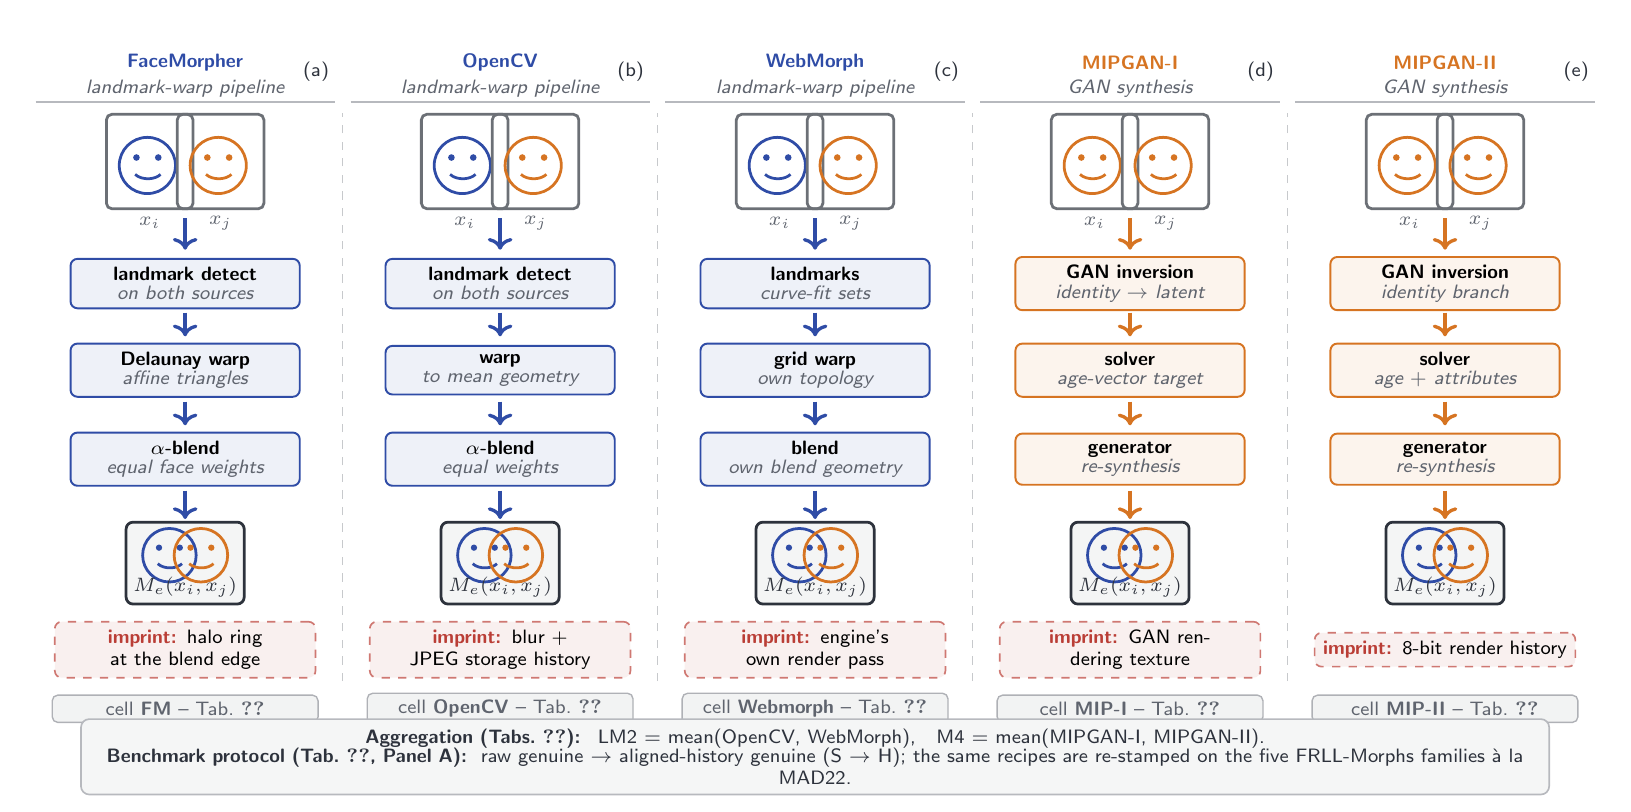
\begin{tikzpicture}[
  x=1cm,y=1cm,
  font=\sffamily,
  every node/.style={align=center, inner sep=1.5pt, outer sep=0pt},
  fline/.style={line width=1.0pt},
  hrule/.style={draw=tzGray!45, line width=0.6pt},
  vsep/.style={draw=tzGray!35, dashed, line width=0.6pt},
  flowlm/.style={->, tzBlue, line width=1.2pt},
  flowgan/.style={->, tzOrange, line width=1.2pt},
  lmchip/.style={draw=tzBlue, fill=tzBlue!8, rounded corners=2.5pt,
                 line width=0.7pt, text width=2.7cm,
                 font=\sffamily\scriptsize, inner sep=3pt},
  ganchip/.style={draw=tzOrange, fill=tzOrange!8, rounded corners=2.5pt,
                  line width=0.7pt, text width=2.7cm,
                  font=\sffamily\scriptsize, inner sep=3pt},
  imprint/.style={draw=tzRed!70, fill=tzRed!8, dashed, rounded corners=2.5pt,
                  line width=0.6pt, text width=3.1cm,
                  font=\sffamily\scriptsize, inner sep=3pt},
  bench/.style={draw=tzGray!50, fill=tzGray!8, rounded corners=2pt,
                line width=0.5pt, text width=3.2cm,
                font=\sffamily\scriptsize, inner sep=2.5pt, text=tzGray},
  pname/.style={font=\sffamily\bfseries\scriptsize},
  ptag/.style={font=\sffamily\scriptsize\itshape, text=tzGray},
  hint/.style={font=\sffamily\scriptsize, text=tzGray},
  stamp/.style={font=\sffamily\scriptsize, text=tzDark},
]
\useasboundingbox (0,0) rectangle (20,9.6);
\definecolor{tzBlue}{RGB}{47,76,166}
\definecolor{tzOrange}{RGB}{214,116,34}
\definecolor{tzGray}{RGB}{95,100,110}
\definecolor{tzDark}{RGB}{45,50,60}
\definecolor{tzRed}{RGB}{186,62,54}

\tikzset{
  % abstract, generic line-art face (identical to teaser's icon)
  picface/.pic={
    \draw[fline, pic actions] (0,0) circle (0.85);
    \fill[pic actions] (-0.33,0.24) circle (0.10);
    \fill[pic actions] (0.33,0.24) circle (0.10);
    \draw[fline, pic actions] (-0.37,-0.27) arc (215:325:0.47 and 0.31);
  },
}

% helper macros: sources pair, morph glyph ---------------------------
\newcommand{\famsources}[2]{% #1 = x center, #2 = flow color
  \begin{scope}[shift={(#1-0.45,7.9)}]
    \draw[fline, tzDark!70, rounded corners=2pt] (-0.55,-0.60) rectangle (0.55,0.60);
    \path (-0.03,-0.05) pic[scale=0.42, #2] {picface};
  \end{scope}
  \begin{scope}[shift={(#1+0.45,7.9)}]
    \draw[fline, tzDark!70, rounded corners=2pt] (-0.55,-0.60) rectangle (0.55,0.60);
    \path (-0.03,-0.05) pic[scale=0.42, tzOrange] {picface};
  \end{scope}
  \node[hint] at (#1-0.45,7.12) {$x_i$};
  \node[hint] at (#1+0.45,7.12) {$x_j$};
}
\newcommand{\fammorph}[1]{% #1 = x center; two contributors + frame
  \begin{scope}[shift={(#1,2.80)}]
    \draw[fline, tzDark, rounded corners=2.5pt, fill=tzDark!5]
      (-0.75,-0.52) rectangle (0.75,0.52);
    \path (-0.20,0.10) pic[scale=0.40, tzBlue] {picface};
    \path (0.20,0.10) pic[scale=0.40, tzOrange] {picface};
    \node[stamp] at (0,-0.30) {\scriptsize$M_e(x_i,x_j)$};
  \end{scope}
}

% ===================== PANEL (a): FaceMorpher ========================
\def\famx{2}
\node[pname, text=tzBlue] at (\famx,9.15) {FaceMorpher};
\node[ptag] at (\famx,8.82) {landmark-warp pipeline};
\draw[hrule] (\famx-1.9,8.66) -- (\famx+1.9,8.66);
\node[stamp, anchor=north east] at (\famx+1.88,9.22) {\scriptsize(a)};
\famsources{\famx}{tzBlue}
\draw[flowlm] (\famx,7.18) -- (\famx,6.78);
\node[lmchip] at (\famx,6.35) {\textbf{landmark detect}\\[-1pt]{\scriptsize\itshape\textcolor{tzGray}{on both sources}}};
\draw[flowlm] (\famx,5.98) -- (\famx,5.68);
\node[lmchip] at (\famx,5.25) {\textbf{Delaunay warp}\\[-1pt]{\scriptsize\itshape\textcolor{tzGray}{affine triangles}}};
\draw[flowlm] (\famx,4.85) -- (\famx,4.55);
\node[lmchip] at (\famx,4.12) {\textbf{$\alpha$-blend}\\[-1pt]{\scriptsize\itshape\textcolor{tzGray}{equal face weights}}};
\draw[flowlm] (\famx,3.72) -- (\famx,3.36);
\fammorph{\famx}
\node[imprint] at (\famx,1.70) {\textcolor{tzRed}{\textbf{imprint:}} halo ring at the blend edge};
\node[bench] at (\famx,0.95) {cell \textbf{FM} -- Tab.~\ref{tab:mad22_results}};

% ===================== PANEL (b): OpenCV =============================
\def\famx{6}
\node[pname, text=tzBlue] at (\famx,9.15) {OpenCV};
\node[ptag] at (\famx,8.82) {landmark-warp pipeline};
\draw[hrule] (\famx-1.9,8.66) -- (\famx+1.9,8.66);
\node[stamp, anchor=north east] at (\famx+1.88,9.22) {\scriptsize(b)};
\famsources{\famx}{tzBlue}
\draw[flowlm] (\famx,7.18) -- (\famx,6.78);
\node[lmchip] at (\famx,6.35) {\textbf{landmark detect}\\[-1pt]{\scriptsize\itshape\textcolor{tzGray}{on both sources}}};
\draw[flowlm] (\famx,5.98) -- (\famx,5.68);
\node[lmchip] at (\famx,5.25) {\textbf{warp}\\[-1pt]{\scriptsize\itshape\textcolor{tzGray}{to mean geometry}}};
\draw[flowlm] (\famx,4.85) -- (\famx,4.55);
\node[lmchip] at (\famx,4.12) {\textbf{$\alpha$-blend}\\[-1pt]{\scriptsize\itshape\textcolor{tzGray}{equal weights}}};
\draw[flowlm] (\famx,3.72) -- (\famx,3.36);
\fammorph{\famx}
\node[imprint] at (\famx,1.70) {\textcolor{tzRed}{\textbf{imprint:}} blur + JPEG storage history};
\node[bench] at (\famx,0.95) {cell \textbf{OpenCV} -- Tab.~\ref{tab:mad22_results}};

% ===================== PANEL (c): WebMorph ===========================
\def\famx{10}
\node[pname, text=tzBlue] at (\famx,9.15) {WebMorph};
\node[ptag] at (\famx,8.82) {landmark-warp pipeline};
\draw[hrule] (\famx-1.9,8.66) -- (\famx+1.9,8.66);
\node[stamp, anchor=north east] at (\famx+1.88,9.22) {\scriptsize(c)};
\famsources{\famx}{tzBlue}
\draw[flowlm] (\famx,7.18) -- (\famx,6.78);
\node[lmchip] at (\famx,6.35) {\textbf{landmarks}\\[-1pt]{\scriptsize\itshape\textcolor{tzGray}{curve-fit sets}}};
\draw[flowlm] (\famx,5.98) -- (\famx,5.68);
\node[lmchip] at (\famx,5.25) {\textbf{grid warp}\\[-1pt]{\scriptsize\itshape\textcolor{tzGray}{own topology}}};
\draw[flowlm] (\famx,4.85) -- (\famx,4.55);
\node[lmchip] at (\famx,4.12) {\textbf{blend}\\[-1pt]{\scriptsize\itshape\textcolor{tzGray}{own blend geometry}}};
\draw[flowlm] (\famx,3.72) -- (\famx,3.36);
\fammorph{\famx}
\node[imprint] at (\famx,1.70) {\textcolor{tzRed}{\textbf{imprint:}} engine's own render pass};
\node[bench] at (\famx,0.95) {cell \textbf{Webmorph} -- Tab.~\ref{tab:mad22_results}};

% ===================== PANEL (d): MIPGAN-I ===========================
\def\famx{14}
\node[pname, text=tzOrange] at (\famx,9.15) {MIPGAN-I};
\node[ptag] at (\famx,8.82) {GAN synthesis};
\draw[hrule] (\famx-1.9,8.66) -- (\famx+1.9,8.66);
\node[stamp, anchor=north east] at (\famx+1.88,9.22) {\scriptsize(d)};
\famsources{\famx}{tzOrange}
\draw[flowgan] (\famx,7.18) -- (\famx,6.78);
\node[ganchip] at (\famx,6.35) {\textbf{GAN inversion}\\[-1pt]{\scriptsize\itshape\textcolor{tzGray}{identity $\to$ latent}}};
\draw[flowgan] (\famx,5.98) -- (\famx,5.68);
\node[ganchip] at (\famx,5.25) {\textbf{solver}\\[-1pt]{\scriptsize\itshape\textcolor{tzGray}{age-vector target}}};
\draw[flowgan] (\famx,4.85) -- (\famx,4.55);
\node[ganchip] at (\famx,4.12) {\textbf{generator}\\[-1pt]{\scriptsize\itshape\textcolor{tzGray}{re-synthesis}}};
\draw[flowgan] (\famx,3.72) -- (\famx,3.36);
\fammorph{\famx}
\node[imprint] at (\famx,1.70) {\textcolor{tzRed}{\textbf{imprint:}} GAN rendering texture};
\node[bench] at (\famx,0.95) {cell \textbf{MIP-I} -- Tab.~\ref{tab:mad22_results}};

% ===================== PANEL (e): MIPGAN-II ==========================
\def\famx{18}
\node[pname, text=tzOrange] at (\famx,9.15) {MIPGAN-II};
\node[ptag] at (\famx,8.82) {GAN synthesis};
\draw[hrule] (\famx-1.9,8.66) -- (\famx+1.9,8.66);
\node[stamp, anchor=north east] at (\famx+1.88,9.22) {\scriptsize(e)};
\famsources{\famx}{tzOrange}
\draw[flowgan] (\famx,7.18) -- (\famx,6.78);
\node[ganchip] at (\famx,6.35) {\textbf{GAN inversion}\\[-1pt]{\scriptsize\itshape\textcolor{tzGray}{identity branch}}};
\draw[flowgan] (\famx,5.98) -- (\famx,5.68);
\node[ganchip] at (\famx,5.25) {\textbf{solver}\\[-1pt]{\scriptsize\itshape\textcolor{tzGray}{age $+$ attributes}}};
\draw[flowgan] (\famx,4.85) -- (\famx,4.55);
\node[ganchip] at (\famx,4.12) {\textbf{generator}\\[-1pt]{\scriptsize\itshape\textcolor{tzGray}{re-synthesis}}};
\draw[flowgan] (\famx,3.72) -- (\famx,3.36);
\fammorph{\famx}
\node[imprint] at (\famx,1.70) {\textcolor{tzRed}{\textbf{imprint:}} 8-bit render history};
\node[bench] at (\famx,0.95) {cell \textbf{MIP-II} -- Tab.~\ref{tab:mad22_results}};

% ------------------------------------------------- panel separations
\foreach \sx in {4,8,12,16}{\draw[vsep] (\sx,1.30) -- (\sx,8.52);}

% ------------------------------------------------ bottom summary strip
\node[draw=tzGray!45, fill=tzGray!6, rounded corners=3pt, line width=0.6pt,
      text width=18.4cm, font=\sffamily\scriptsize, inner sep=3.5pt,
      text=tzDark] at (10,0.34)
 {{\textbf{Aggregation (Tabs.~\ref{tab:mad22_results}):\ } LM2~$=$~mean(OpenCV,~WebMorph),\quad M4~$=$~mean(MIPGAN-I,~MIPGAN-II).}\\[-1pt]
  {\textbf{Benchmark protocol (Tab.~\ref{tab:mad22_results}, Panel~A):\ } raw genuine $\rightarrow$ aligned-history genuine (S~$\rightarrow$~H); the same recipes are re-stamped on the five FRLL-Morphs families \`a la MAD22.}};

\end{tikzpicture}}%
\captionsetup{hypcap=false}
\caption{The five morph families covered by the shortcut analysis (schematic; no real-face imagery).
\textbf{Blue:} landmark-warping pipelines -- landmark detection, geometric warp, blending -- that share the construction but differ in blend geometry and post-processing (FaceMorpher's halo ring, OpenCV's blur/JPEG storage history, WebMorph's own warp and blend field).
\textbf{Orange:} GAN synthesis in two variants (MIPGAN-I, MIPGAN-II).
Each panel annotates the processing trace most likely to \emph{imprint} -- the imprint a shortcut detector can latch onto without seeing two identities.
All families are benchmarked in Table~\ref{tab:mad22_results} under the raw-to-aligned-history genuine protocol (S~$\to$~H, Panel~A); aggregations average OpenCV$+$WebMorph into LM2 and MIPGAN-I$/$II into M4.
The same recipes were re-applied to rebuild the five FRLL-Morphs families \`a la MAD22 (Table~\ref{tab:frll_results}).}
\label{fig:families}
\end{figure*}

%%
%% Fig -- real MAD22 morph-family figure (figures/families_photos.tex):
%% actual corpus images, one identity-matched A|morph|B row per family with
%% per-family shortcut labels; ENABLED below, discussed in results.tex.
% =====================================================================
% fig:families_photos — compact FULL-WIDTH photo figure (figure*):
% single row: leftmost Source A, then one representative
% identity-matched MAD22 morph per family (FaceMorpher, OpenCV,
% WebMorph, MIPGAN-I, MIPGAN-II), rightmost Source B (010_03). All
% seven panels come from the same corrected corpus rows of one shared
% contributor pair (A = 001_03, B = 010_03); every morph in the row
% blends exactly these two contributors.
%
% Image source: native rows of the corrected MAD22 corpus
%   /mnt/t7/smad_heldout/mad22_canonical_E7_inputs_v3_20261109T113746Z
%   (sha256 of each panel preserved through downsampling in the
%   supplementary build manifest; volumes as in tab:mad22_results).
% REAL corpus imagery (unlike figures/teaser.tex and
% figures/families.tex). Two people per row, adults only.
% The FaceMorpher image retains its released generator watermark.
% Every panel is a genuinely retained row of the corrected
% benchmark; selection is descriptive only and part of no claim.
%
% Layout: no \resizebox, no node-nested inline \tikz (both are
% known hazards in this project); plain tabular + \includegraphics
% + \parbox labels. Smallest text: \tiny on \scriptsize panels.
% =====================================================================
\begin{figure*}[t]
\centering
\setlength{\tabcolsep}{2pt}%
\begin{tabular}{@{}c@{\hspace{3pt}}c@{\hspace{3pt}}c@{\hspace{3pt}}c@{\hspace{3pt}}c@{\hspace{3pt}}c@{\hspace{3pt}}c@{}}
  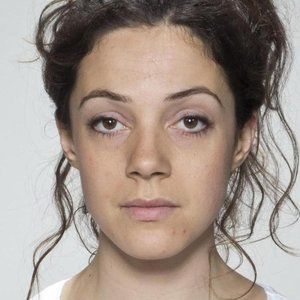
\includegraphics[width=0.125\textwidth]{families_photos/person001_photo.jpg} &
  \frame{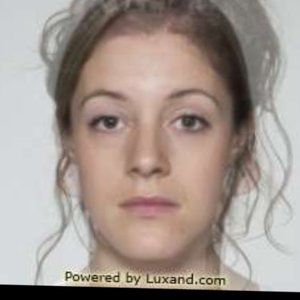
\includegraphics[width=0.125\textwidth]{families_photos/morph_facemorpher.jpg}} &
  \frame{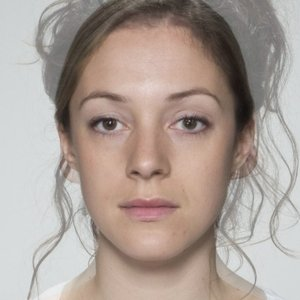
\includegraphics[width=0.125\textwidth]{families_photos/morph_opencv.jpg}} &
  \frame{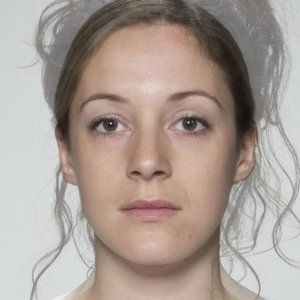
\includegraphics[width=0.125\textwidth]{families_photos/morph_webmorph.jpg}} &
  \frame{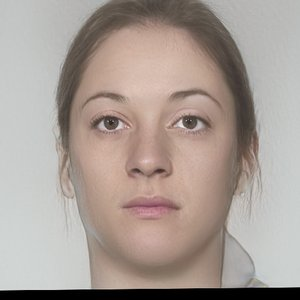
\includegraphics[width=0.125\textwidth]{families_photos/morph_mipgan1.jpg}} &
  \frame{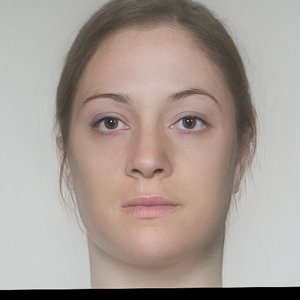
\includegraphics[width=0.125\textwidth]{families_photos/morph_mipgan2.jpg}} &
  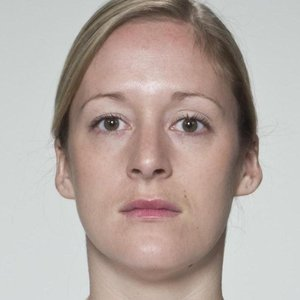
\includegraphics[width=0.125\textwidth]{families_photos/person010_photo.jpg}\\[3pt]
  {\tiny\sffamily\textbf{Source A}} &
  {\tiny\sffamily\textbf{FaceMorpher}} &
  {\tiny\sffamily\textbf{OpenCV}} &
  {\tiny\sffamily\textbf{WebMorph}} &
  {\tiny\sffamily\textbf{MIPGAN-I}} &
  {\tiny\sffamily\textbf{MIPGAN-II}} &
  {\tiny\sffamily\textbf{Source B}}\\[-1pt]
  {\tiny\sffamily contributor 001\_03} &
  \parbox[t]{0.135\textwidth}{\centering\tiny\sffamily halo ring + sharpness/energy} &
  \parbox[t]{0.135\textwidth}{\centering\tiny\sffamily halo + warp-only surround} &
  \parbox[t]{0.135\textwidth}{\centering\tiny\sffamily halo ring + illumination/pose} &
  \parbox[t]{0.135\textwidth}{\centering\tiny\sffamily GAN fingerprint response} &
  \parbox[t]{0.135\textwidth}{\centering\tiny\sffamily GAN fingerprint + sharpness} &
  {\tiny\sffamily contributor 010\_03}\\
\end{tabular}
\caption{Real examples of the five MAD22 morph families analyzed in
Sections~\ref{sec:matched_controls} and~\ref{sec:benchmark_results}. Every morph is a
genuine blend of the same two contributor photographs shown at the ends of
the row (A = 001\_03, B = 010\_03), drawn from the corrected benchmark;
the shortcut label under each panel names the non-identity trait our
instruments isolate for that family. Descriptive illustration only; not a
benchmark claim.}
\label{fig:families_photos}
\end{figure*}

%%
%% Fig -- shortcut-traits verdict map (figures/shortcuts_overview.tex):
%% TikZ requires \begin{figure}[t]\centering\input{...}\caption...\end{figure}
%% wrapping, ENABLED below (tall single-column figure).
\begin{figure}[tbp]
\centering
% fig:shortcuts_overview -- conceptual taxonomy of non-identity shortcut traits.
% Single-column TikZ (design width 8.2 cm = \columnwidth), native-size fonts,
% no \resizebox, no node-nested \tikz, no \newcommand-pics. Schematic glyphs
% only, no real-face imagery. Suggested include (figure env + caption live in
% main.tex):
%   \begin{figure}[t]\centering% fig:shortcuts_overview -- conceptual taxonomy of non-identity shortcut traits.
% Single-column TikZ (design width 8.2 cm = \columnwidth), native-size fonts,
% no \resizebox, no node-nested \tikz, no \newcommand-pics. Schematic glyphs
% only, no real-face imagery. Suggested include (figure env + caption live in
% main.tex):
%   \begin{figure}[t]\centering% fig:shortcuts_overview -- conceptual taxonomy of non-identity shortcut traits.
% Single-column TikZ (design width 8.2 cm = \columnwidth), native-size fonts,
% no \resizebox, no node-nested \tikz, no \newcommand-pics. Schematic glyphs
% only, no real-face imagery. Suggested include (figure env + caption live in
% main.tex):
%   \begin{figure}[t]\centering\input{figures/shortcuts_overview.tex}...\end{figure}
% Verdicts are the registered reads from results.tex; do not paraphrase stronger.
\centering
\definecolor{tzBlue}{RGB}{47,76,166}
\definecolor{tzOrange}{RGB}{214,116,34}
\definecolor{tzGray}{RGB}{95,100,110}
\definecolor{tzDark}{RGB}{45,50,60}
\begin{tikzpicture}[
  x=1cm,y=1cm,
  font=\sffamily,
  every node/.style={align=left, inner sep=1.5pt, outer sep=0pt},
  fline/.style={line width=1.0pt},
  hrule/.style={draw=tzGray!45, line width=0.6pt},
  boxR/.style={draw=tzBlue, fill=tzBlue!8, rounded corners=3pt, line width=0.8pt},
  fam/.style={draw=tzBlue!60, fill=white, rounded corners=3pt, line width=0.7pt},
  head/.style={anchor=west, font=\sffamily\bfseries\footnotesize, text=tzBlue},
  famHead/.style={anchor=north west, font=\sffamily\bfseries\scriptsize, text=tzDark},
  sub/.style={anchor=north west, font=\sffamily\tiny, text=tzGray},
  trait/.style={anchor=north west, font=\sffamily\tiny, text=tzDark},
  vEst/.style={draw=tzOrange, fill=tzOrange!15, rounded corners=2pt, line width=0.7pt,
               font=\sffamily\tiny, text=tzDark},
  vAtt/.style={draw=tzBlue, fill=tzBlue!8, rounded corners=2pt, line width=0.7pt,
               font=\sffamily\tiny, text=tzDark},
  vInc/.style={draw=tzGray, dashed, fill=tzGray!6, rounded corners=2pt, line width=0.6pt,
               font=\sffamily\tiny, text=tzGray},
  hint/.style={anchor=north west, font=\sffamily\tiny, text=tzGray},
  spoke/.style={->, tzGray!80, line width=0.9pt},
  qlab/.style={font=\sffamily\tiny\itshape, text=tzGray},
]
\useasboundingbox (-0.15,0.05) rectangle (8.35,11.50);

% ============================================================== header
\node[head] at (-0.1,11.28) {What a single-image morph detector can respond to};
\draw[hrule] (-0.05,11.03) -- (8.25,11.03);

% ============================================================== hub node
\draw[boxR] (2.40,7.05) rectangle (5.80,8.00);
\begin{scope}[shift={(3.02,7.52)}]
  \draw[fline, tzBlue] (-0.10,0) circle (0.24);
  \fill[tzBlue] (-0.21,0.07) circle (0.028);
  \fill[tzBlue] (0.01,0.07) circle (0.028);
  \draw[fline, tzBlue] (-0.21,-0.08) arc (215:325:0.13 and 0.09);
  \draw[fline, tzOrange] (0.24,0) circle (0.24);
  \fill[tzOrange] (0.13,0.07) circle (0.028);
  \fill[tzOrange] (0.35,0.07) circle (0.028);
  \draw[fline, tzOrange] (0.13,-0.08) arc (215:325:0.13 and 0.09);
\end{scope}
\node[anchor=west, font=\sffamily\tiny\bfseries, text=tzDark] at (3.55,7.66)
  {morph candidate};
\node[anchor=west, font=\sffamily\tiny, text=tzGray] at (3.55,7.38)
  {single-image (S-MAD) decision};

% ------------------------------------- radiating spokes: hub to trait groups
% top-left
\draw[spoke] (3.05,8.00) -- (2.55,8.36);
% top-right
\draw[spoke] (5.15,8.00) -- (5.65,8.36);
% bottom-left
\draw[spoke] (3.05,7.05) -- (2.55,6.74);
% bottom-right
\draw[spoke] (5.15,7.05) -- (5.65,6.74);
% center: down the corridor between the lower boxes to (5) contributor
\draw[spoke] (4.10,7.05) -- (4.10,3.41);

% ================================================================ 1 TL
\draw[fam] (0.00,8.40) rectangle (3.90,10.78);
\node[famHead] at (0.10,10.73) {(1) Processing \& storage};
\node[sub] at (0.10,10.44) {isolation instruments: MF + CB};
\node[trait] at (0.10,10.16)
  {\textbf{shrink-\&-enlarge history} $256\!\to\!80\!\to\!224$ {\color{tzBlue}\textbf{[MF]}}};
\node[vEst, anchor=north west, text width=3.42cm] at (0.10,9.90)
  {sufficient for 0.0\% EER on native MorDIFF, 10/10 networks, with no morphs in training};
\node[trait] at (0.10,9.16) {\textbf{JPEG / storage size} {\color{tzBlue}\textbf{[MF, CB]}}};
\node[vInc, anchor=north west, text width=3.42cm] at (0.10,8.90)
  {registered combined verdict inconclusive (5/5 trained, 3/5 untrained seeds); false alarms attenuated, not removed};

% ================================================================ 2 TR
\draw[fam] (4.30,8.40) rectangle (8.20,10.78);
\node[famHead] at (4.40,10.73) {(2) Rendering};
\node[sub] at (4.40,10.44) {isolation instrument: MC};
\node[trait] at (4.40,10.16)
  {\textbf{one-photo generative reconstruction} {\color{tzBlue}\textbf{[MC]}}};
\node[vEst, anchor=north west, text width=3.42cm] at (4.40,9.90)
  {render-path verdict \emph{used} (5/5 seeds); 78--90\% of renders flagged despite no second identity};
\node[trait, text width=3.42cm] at (4.40,9.16)
  {\textbf{GAN fingerprints} (MIPGAN, StyleGAN-style) {\color{tzBlue}\textbf{[MC]}}};
\node[vInc, anchor=north west, text width=3.42cm] at (4.40,8.90)
  {inconclusive: low GAN-family EER not established as morph-specific};

% ================================================================ 3 BL
\draw[fam] (0.00,4.25) rectangle (3.90,6.70);
\node[famHead] at (0.10,6.65) {(3) Blending};
\node[sub] at (0.10,6.36) {isolation instrument: MC};
\node[trait, text width=3.42cm] at (0.10,6.08)
  {\textbf{warp geometric trace}, \textbf{tool halo ring},\\[1pt]
   \textbf{noise / variance averaging} {\color{tzBlue}\textbf{[MC]}}};
\node[vInc, anchor=north west, text width=3.42cm] at (0.10,5.44)
  {blend vs warp: $+0.011$ AUC [$-$0.010, 0.031] --- registered: inconclusive};
\node[hint] at (0.10,4.78)
  {low-level statistics: 0.925 / 0.917 AUC (viable)};

% ================================================================ 4 BR
\draw[fam] (4.30,4.25) rectangle (8.20,6.70);
\node[famHead] at (4.40,6.65) {(4) Splice construction};
\node[sub] at (4.40,6.36) {isolation instruments: MC + CB};
\node[trait] at (4.40,6.08) {\textbf{insertion seam} {\color{tzBlue}\textbf{[MC]}}};
\node[vAtt, anchor=north west, text width=3.42cm] at (4.40,5.84)
  {seam-only negative: labels not reproduced from the seam alone};
\node[trait] at (4.40,5.24) {\textbf{same-person splice} {\color{tzBlue}\textbf{[CB]}}};
\node[vAtt, anchor=north west, text width=3.42cm] at (4.40,5.00)
  {flags 70--74\% $\to$ 36--41\% at the own rule: attenuated, still flagged};
\node[vEst, anchor=north west, text width=3.42cm] at (4.40,4.48)
  {full recipe gain $+0.048$ AUC, 5/5 seeds (count-balanced)};

% ================================================================ 5 band
\draw[fam] (0.00,1.95) rectangle (8.20,3.35);
\node[famHead] at (0.10,3.30) {(5) Contributor dependence};
\node[sub] at (3.40,3.30) {isolation instruments: MC + CB};
\node[trait, text width=3.95cm] at (0.10,2.98)
  {a same-person morph blends two photographs of \emph{one} identity:\\[1pt]
   verification helps that person only.};
\node[vInc, anchor=west, text width=3.30cm] at (4.40,2.62)
  {85\% of same-person morphs still flagged --- identity-specific detection: open};

% ============================================================== legend
\node[vEst] at (1.42,1.58) {registered: shortcut used / sufficient};
\node[vAtt] at (3.95,1.58) {attenuated, not removed};
\node[vInc] at (6.62,1.58) {registered: inconclusive / open};
\node[font=\sffamily\tiny, text=tzDark] at (4.10,1.06)
  {\textbf{MF}\, morph-free training\quad
   \textbf{MC}\, matched-control ladder\quad
   \textbf{CB}\, count-balanced training ablation};
\node[qlab] at (4.10,0.52)
  {verdicts are the registered reads of Sec.~4; passing one control does not certify the next};

\end{tikzpicture}
...\end{figure}
% Verdicts are the registered reads from results.tex; do not paraphrase stronger.
\centering
\definecolor{tzBlue}{RGB}{47,76,166}
\definecolor{tzOrange}{RGB}{214,116,34}
\definecolor{tzGray}{RGB}{95,100,110}
\definecolor{tzDark}{RGB}{45,50,60}
\begin{tikzpicture}[
  x=1cm,y=1cm,
  font=\sffamily,
  every node/.style={align=left, inner sep=1.5pt, outer sep=0pt},
  fline/.style={line width=1.0pt},
  hrule/.style={draw=tzGray!45, line width=0.6pt},
  boxR/.style={draw=tzBlue, fill=tzBlue!8, rounded corners=3pt, line width=0.8pt},
  fam/.style={draw=tzBlue!60, fill=white, rounded corners=3pt, line width=0.7pt},
  head/.style={anchor=west, font=\sffamily\bfseries\footnotesize, text=tzBlue},
  famHead/.style={anchor=north west, font=\sffamily\bfseries\scriptsize, text=tzDark},
  sub/.style={anchor=north west, font=\sffamily\tiny, text=tzGray},
  trait/.style={anchor=north west, font=\sffamily\tiny, text=tzDark},
  vEst/.style={draw=tzOrange, fill=tzOrange!15, rounded corners=2pt, line width=0.7pt,
               font=\sffamily\tiny, text=tzDark},
  vAtt/.style={draw=tzBlue, fill=tzBlue!8, rounded corners=2pt, line width=0.7pt,
               font=\sffamily\tiny, text=tzDark},
  vInc/.style={draw=tzGray, dashed, fill=tzGray!6, rounded corners=2pt, line width=0.6pt,
               font=\sffamily\tiny, text=tzGray},
  hint/.style={anchor=north west, font=\sffamily\tiny, text=tzGray},
  spoke/.style={->, tzGray!80, line width=0.9pt},
  qlab/.style={font=\sffamily\tiny\itshape, text=tzGray},
]
\useasboundingbox (-0.15,0.05) rectangle (8.35,11.50);

% ============================================================== header
\node[head] at (-0.1,11.28) {What a single-image morph detector can respond to};
\draw[hrule] (-0.05,11.03) -- (8.25,11.03);

% ============================================================== hub node
\draw[boxR] (2.40,7.05) rectangle (5.80,8.00);
\begin{scope}[shift={(3.02,7.52)}]
  \draw[fline, tzBlue] (-0.10,0) circle (0.24);
  \fill[tzBlue] (-0.21,0.07) circle (0.028);
  \fill[tzBlue] (0.01,0.07) circle (0.028);
  \draw[fline, tzBlue] (-0.21,-0.08) arc (215:325:0.13 and 0.09);
  \draw[fline, tzOrange] (0.24,0) circle (0.24);
  \fill[tzOrange] (0.13,0.07) circle (0.028);
  \fill[tzOrange] (0.35,0.07) circle (0.028);
  \draw[fline, tzOrange] (0.13,-0.08) arc (215:325:0.13 and 0.09);
\end{scope}
\node[anchor=west, font=\sffamily\tiny\bfseries, text=tzDark] at (3.55,7.66)
  {morph candidate};
\node[anchor=west, font=\sffamily\tiny, text=tzGray] at (3.55,7.38)
  {single-image (S-MAD) decision};

% ------------------------------------- radiating spokes: hub to trait groups
% top-left
\draw[spoke] (3.05,8.00) -- (2.55,8.36);
% top-right
\draw[spoke] (5.15,8.00) -- (5.65,8.36);
% bottom-left
\draw[spoke] (3.05,7.05) -- (2.55,6.74);
% bottom-right
\draw[spoke] (5.15,7.05) -- (5.65,6.74);
% center: down the corridor between the lower boxes to (5) contributor
\draw[spoke] (4.10,7.05) -- (4.10,3.41);

% ================================================================ 1 TL
\draw[fam] (0.00,8.40) rectangle (3.90,10.78);
\node[famHead] at (0.10,10.73) {(1) Processing \& storage};
\node[sub] at (0.10,10.44) {isolation instruments: MF + CB};
\node[trait] at (0.10,10.16)
  {\textbf{shrink-\&-enlarge history} $256\!\to\!80\!\to\!224$ {\color{tzBlue}\textbf{[MF]}}};
\node[vEst, anchor=north west, text width=3.42cm] at (0.10,9.90)
  {sufficient for 0.0\% EER on native MorDIFF, 10/10 networks, with no morphs in training};
\node[trait] at (0.10,9.16) {\textbf{JPEG / storage size} {\color{tzBlue}\textbf{[MF, CB]}}};
\node[vInc, anchor=north west, text width=3.42cm] at (0.10,8.90)
  {registered combined verdict inconclusive (5/5 trained, 3/5 untrained seeds); false alarms attenuated, not removed};

% ================================================================ 2 TR
\draw[fam] (4.30,8.40) rectangle (8.20,10.78);
\node[famHead] at (4.40,10.73) {(2) Rendering};
\node[sub] at (4.40,10.44) {isolation instrument: MC};
\node[trait] at (4.40,10.16)
  {\textbf{one-photo generative reconstruction} {\color{tzBlue}\textbf{[MC]}}};
\node[vEst, anchor=north west, text width=3.42cm] at (4.40,9.90)
  {render-path verdict \emph{used} (5/5 seeds); 78--90\% of renders flagged despite no second identity};
\node[trait, text width=3.42cm] at (4.40,9.16)
  {\textbf{GAN fingerprints} (MIPGAN, StyleGAN-style) {\color{tzBlue}\textbf{[MC]}}};
\node[vInc, anchor=north west, text width=3.42cm] at (4.40,8.90)
  {inconclusive: low GAN-family EER not established as morph-specific};

% ================================================================ 3 BL
\draw[fam] (0.00,4.25) rectangle (3.90,6.70);
\node[famHead] at (0.10,6.65) {(3) Blending};
\node[sub] at (0.10,6.36) {isolation instrument: MC};
\node[trait, text width=3.42cm] at (0.10,6.08)
  {\textbf{warp geometric trace}, \textbf{tool halo ring},\\[1pt]
   \textbf{noise / variance averaging} {\color{tzBlue}\textbf{[MC]}}};
\node[vInc, anchor=north west, text width=3.42cm] at (0.10,5.44)
  {blend vs warp: $+0.011$ AUC [$-$0.010, 0.031] --- registered: inconclusive};
\node[hint] at (0.10,4.78)
  {low-level statistics: 0.925 / 0.917 AUC (viable)};

% ================================================================ 4 BR
\draw[fam] (4.30,4.25) rectangle (8.20,6.70);
\node[famHead] at (4.40,6.65) {(4) Splice construction};
\node[sub] at (4.40,6.36) {isolation instruments: MC + CB};
\node[trait] at (4.40,6.08) {\textbf{insertion seam} {\color{tzBlue}\textbf{[MC]}}};
\node[vAtt, anchor=north west, text width=3.42cm] at (4.40,5.84)
  {seam-only negative: labels not reproduced from the seam alone};
\node[trait] at (4.40,5.24) {\textbf{same-person splice} {\color{tzBlue}\textbf{[CB]}}};
\node[vAtt, anchor=north west, text width=3.42cm] at (4.40,5.00)
  {flags 70--74\% $\to$ 36--41\% at the own rule: attenuated, still flagged};
\node[vEst, anchor=north west, text width=3.42cm] at (4.40,4.48)
  {full recipe gain $+0.048$ AUC, 5/5 seeds (count-balanced)};

% ================================================================ 5 band
\draw[fam] (0.00,1.95) rectangle (8.20,3.35);
\node[famHead] at (0.10,3.30) {(5) Contributor dependence};
\node[sub] at (3.40,3.30) {isolation instruments: MC + CB};
\node[trait, text width=3.95cm] at (0.10,2.98)
  {a same-person morph blends two photographs of \emph{one} identity:\\[1pt]
   verification helps that person only.};
\node[vInc, anchor=west, text width=3.30cm] at (4.40,2.62)
  {85\% of same-person morphs still flagged --- identity-specific detection: open};

% ============================================================== legend
\node[vEst] at (1.42,1.58) {registered: shortcut used / sufficient};
\node[vAtt] at (3.95,1.58) {attenuated, not removed};
\node[vInc] at (6.62,1.58) {registered: inconclusive / open};
\node[font=\sffamily\tiny, text=tzDark] at (4.10,1.06)
  {\textbf{MF}\, morph-free training\quad
   \textbf{MC}\, matched-control ladder\quad
   \textbf{CB}\, count-balanced training ablation};
\node[qlab] at (4.10,0.52)
  {verdicts are the registered reads of Sec.~4; passing one control does not certify the next};

\end{tikzpicture}
...\end{figure}
% Verdicts are the registered reads from results.tex; do not paraphrase stronger.
\centering
\definecolor{tzBlue}{RGB}{47,76,166}
\definecolor{tzOrange}{RGB}{214,116,34}
\definecolor{tzGray}{RGB}{95,100,110}
\definecolor{tzDark}{RGB}{45,50,60}
\begin{tikzpicture}[
  x=1cm,y=1cm,
  font=\sffamily,
  every node/.style={align=left, inner sep=1.5pt, outer sep=0pt},
  fline/.style={line width=1.0pt},
  hrule/.style={draw=tzGray!45, line width=0.6pt},
  boxR/.style={draw=tzBlue, fill=tzBlue!8, rounded corners=3pt, line width=0.8pt},
  fam/.style={draw=tzBlue!60, fill=white, rounded corners=3pt, line width=0.7pt},
  head/.style={anchor=west, font=\sffamily\bfseries\footnotesize, text=tzBlue},
  famHead/.style={anchor=north west, font=\sffamily\bfseries\scriptsize, text=tzDark},
  sub/.style={anchor=north west, font=\sffamily\tiny, text=tzGray},
  trait/.style={anchor=north west, font=\sffamily\tiny, text=tzDark},
  vEst/.style={draw=tzOrange, fill=tzOrange!15, rounded corners=2pt, line width=0.7pt,
               font=\sffamily\tiny, text=tzDark},
  vAtt/.style={draw=tzBlue, fill=tzBlue!8, rounded corners=2pt, line width=0.7pt,
               font=\sffamily\tiny, text=tzDark},
  vInc/.style={draw=tzGray, dashed, fill=tzGray!6, rounded corners=2pt, line width=0.6pt,
               font=\sffamily\tiny, text=tzGray},
  hint/.style={anchor=north west, font=\sffamily\tiny, text=tzGray},
  spoke/.style={->, tzGray!80, line width=0.9pt},
  qlab/.style={font=\sffamily\tiny\itshape, text=tzGray},
]
\useasboundingbox (-0.15,0.05) rectangle (8.35,11.50);

% ============================================================== header
\node[head] at (-0.1,11.28) {What a single-image morph detector can respond to};
\draw[hrule] (-0.05,11.03) -- (8.25,11.03);

% ============================================================== hub node
\draw[boxR] (2.40,7.05) rectangle (5.80,8.00);
\begin{scope}[shift={(3.02,7.52)}]
  \draw[fline, tzBlue] (-0.10,0) circle (0.24);
  \fill[tzBlue] (-0.21,0.07) circle (0.028);
  \fill[tzBlue] (0.01,0.07) circle (0.028);
  \draw[fline, tzBlue] (-0.21,-0.08) arc (215:325:0.13 and 0.09);
  \draw[fline, tzOrange] (0.24,0) circle (0.24);
  \fill[tzOrange] (0.13,0.07) circle (0.028);
  \fill[tzOrange] (0.35,0.07) circle (0.028);
  \draw[fline, tzOrange] (0.13,-0.08) arc (215:325:0.13 and 0.09);
\end{scope}
\node[anchor=west, font=\sffamily\tiny\bfseries, text=tzDark] at (3.55,7.66)
  {morph candidate};
\node[anchor=west, font=\sffamily\tiny, text=tzGray] at (3.55,7.38)
  {single-image (S-MAD) decision};

% ------------------------------------- radiating spokes: hub to trait groups
% top-left
\draw[spoke] (3.05,8.00) -- (2.55,8.36);
% top-right
\draw[spoke] (5.15,8.00) -- (5.65,8.36);
% bottom-left
\draw[spoke] (3.05,7.05) -- (2.55,6.74);
% bottom-right
\draw[spoke] (5.15,7.05) -- (5.65,6.74);
% center: down the corridor between the lower boxes to (5) contributor
\draw[spoke] (4.10,7.05) -- (4.10,3.41);

% ================================================================ 1 TL
\draw[fam] (0.00,8.40) rectangle (3.90,10.78);
\node[famHead] at (0.10,10.73) {(1) Processing \& storage};
\node[sub] at (0.10,10.44) {isolation instruments: MF + CB};
\node[trait] at (0.10,10.16)
  {\textbf{shrink-\&-enlarge history} $256\!\to\!80\!\to\!224$ {\color{tzBlue}\textbf{[MF]}}};
\node[vEst, anchor=north west, text width=3.42cm] at (0.10,9.90)
  {sufficient for 0.0\% EER on native MorDIFF, 10/10 networks, with no morphs in training};
\node[trait] at (0.10,9.16) {\textbf{JPEG / storage size} {\color{tzBlue}\textbf{[MF, CB]}}};
\node[vInc, anchor=north west, text width=3.42cm] at (0.10,8.90)
  {registered combined verdict inconclusive (5/5 trained, 3/5 untrained seeds); false alarms attenuated, not removed};

% ================================================================ 2 TR
\draw[fam] (4.30,8.40) rectangle (8.20,10.78);
\node[famHead] at (4.40,10.73) {(2) Rendering};
\node[sub] at (4.40,10.44) {isolation instrument: MC};
\node[trait] at (4.40,10.16)
  {\textbf{one-photo generative reconstruction} {\color{tzBlue}\textbf{[MC]}}};
\node[vEst, anchor=north west, text width=3.42cm] at (4.40,9.90)
  {render-path verdict \emph{used} (5/5 seeds); 78--90\% of renders flagged despite no second identity};
\node[trait, text width=3.42cm] at (4.40,9.16)
  {\textbf{GAN fingerprints} (MIPGAN, StyleGAN-style) {\color{tzBlue}\textbf{[MC]}}};
\node[vInc, anchor=north west, text width=3.42cm] at (4.40,8.90)
  {inconclusive: low GAN-family EER not established as morph-specific};

% ================================================================ 3 BL
\draw[fam] (0.00,4.25) rectangle (3.90,6.70);
\node[famHead] at (0.10,6.65) {(3) Blending};
\node[sub] at (0.10,6.36) {isolation instrument: MC};
\node[trait, text width=3.42cm] at (0.10,6.08)
  {\textbf{warp geometric trace}, \textbf{tool halo ring},\\[1pt]
   \textbf{noise / variance averaging} {\color{tzBlue}\textbf{[MC]}}};
\node[vInc, anchor=north west, text width=3.42cm] at (0.10,5.44)
  {blend vs warp: $+0.011$ AUC [$-$0.010, 0.031] --- registered: inconclusive};
\node[hint] at (0.10,4.78)
  {low-level statistics: 0.925 / 0.917 AUC (viable)};

% ================================================================ 4 BR
\draw[fam] (4.30,4.25) rectangle (8.20,6.70);
\node[famHead] at (4.40,6.65) {(4) Splice construction};
\node[sub] at (4.40,6.36) {isolation instruments: MC + CB};
\node[trait] at (4.40,6.08) {\textbf{insertion seam} {\color{tzBlue}\textbf{[MC]}}};
\node[vAtt, anchor=north west, text width=3.42cm] at (4.40,5.84)
  {seam-only negative: labels not reproduced from the seam alone};
\node[trait] at (4.40,5.24) {\textbf{same-person splice} {\color{tzBlue}\textbf{[CB]}}};
\node[vAtt, anchor=north west, text width=3.42cm] at (4.40,5.00)
  {flags 70--74\% $\to$ 36--41\% at the own rule: attenuated, still flagged};
\node[vEst, anchor=north west, text width=3.42cm] at (4.40,4.48)
  {full recipe gain $+0.048$ AUC, 5/5 seeds (count-balanced)};

% ================================================================ 5 band
\draw[fam] (0.00,1.95) rectangle (8.20,3.35);
\node[famHead] at (0.10,3.30) {(5) Contributor dependence};
\node[sub] at (3.40,3.30) {isolation instruments: MC + CB};
\node[trait, text width=3.95cm] at (0.10,2.98)
  {a same-person morph blends two photographs of \emph{one} identity:\\[1pt]
   verification helps that person only.};
\node[vInc, anchor=west, text width=3.30cm] at (4.40,2.62)
  {85\% of same-person morphs still flagged --- identity-specific detection: open};

% ============================================================== legend
\node[vEst] at (1.42,1.58) {registered: shortcut used / sufficient};
\node[vAtt] at (3.95,1.58) {attenuated, not removed};
\node[vInc] at (6.62,1.58) {registered: inconclusive / open};
\node[font=\sffamily\tiny, text=tzDark] at (4.10,1.06)
  {\textbf{MF}\, morph-free training\quad
   \textbf{MC}\, matched-control ladder\quad
   \textbf{CB}\, count-balanced training ablation};
\node[qlab] at (4.10,0.52)
  {verdicts are the registered reads of Sec.~4; passing one control does not certify the next};

\end{tikzpicture}

\caption{A verdict map of non-identity shortcut traits in single-image morph detection. A morph candidate (center) can be separated from genuine photographs by traits that have nothing to do with combining two identities. The trait groups are those our instruments isolate: processing and storage (morph-free training reaches 0.0\% EER on the native MorDIFF cell), rendering (the render path alone is a registered \emph{used} cue), blending (the matched blend gain is inconclusive), splice construction (matched negatives attenuate, but do not remove, same-person splice flags), and contributor dependence (still open). Each trait carries its isolating instrument: morph-free training (MF), the matched-control ladder (MC), or a count-balanced ablation (CB).}
\label{fig:shortcuts_overview}
\end{figure}
%%
% (End OPTIONAL FIGURE INCLUDES)
%
\section{Related Work}
\label{sec:related}
\paragraph{Detection settings: S-MAD and D-MAD.}
Following the MAD survey taxonomy~\cite{venkatesh2021survey}, differential MAD (D-MAD) scores a suspected image against a trusted live capture, and single-image MAD (S-MAD) scores the suspected image alone. This paper operates in the S-MAD setting throughout: enrollment-time screening has no trusted reference, and every control, training run and read below scores single images.

\paragraph{Morph generation and attack detection.}
Face morphing can make an enrollment image resemble multiple contributors~\cite{ferrara2014magic}. SYN-MAD evaluates synthetic-to-real transfer~\cite{huber2022synmad}; SMDD supplies synthetic-only training~\cite{damer2022smdd}. MIPGAN uses identity-constrained GAN synthesis~\cite{zhang2021mipgan}, while MorDIFF interpolates diffusion-autoencoder representations~\cite{damer2023mordiff}. Each also changes reconstruction or processing history. Detecting such a pipeline is therefore distinct from detecting two identities, and neither implies a successful recognition attack. Our controls retain more of the construction in common without assuming that this removes every low-level difference.

\paragraph{Foundation models and synthetic supervision.}
CLIP~\cite{radford2021clip} and LoRA~\cite{hu2022lora} already underpin MADation's morph detector~\cite{caldeira2025madation}. We study training examples and evaluation, not a new backbone; even with fixed optimization, removals can alter balance, repetition and diversity. SelfMAD simulates pixel/frequency morph artifacts~\cite{ivanovska2025selfmad}. SelfMAD++ adds a CLIP model, local features and segmentation~\cite{ivanovska2026selfmadpp}; our released SelfMAD comparison is not a comparison with SelfMAD++. Paired controls complement these architecture and augmentation approaches by testing what their scores support.

\paragraph{Shortcut and blending evidence.}
Shortcut learning uses predictive rules that can fail beyond benchmark conditions~\cite{geirhos2020shortcut}. MAD processing differences include resampling, storage, reconstruction and boundaries. Print--scan degradation across devices~\cite{paulo2026printed} motivates acquisition-shift tests; our controls additionally ask whether processing activates a detector without a second identity. Neither perturbation sensitivity nor benchmark accuracy identifies every decision mechanism.

Face X-ray learns blending boundaries~\cite{li2020facexray}; Self-Blended Images generate forgery supervision from single pristine images~\cite{shiohara2022sbi}. Their target is forgery traces. Our same-person and seam-only negatives test whether selected traces suffice for a two-contributor label. A self-blend can thus be useful forgery supervision and a useful contributor-dependence control. Processing-only supervision, matched constructions and training ablations test specified explanations, without certifying identity recognition or eliminating texture, noise averaging, geometry and surround cues.


\section{Disentangling Morphing from Shortcuts}
\label{sec:controlled_eval}

Conventional single-image morphing attack detection (S-MAD)
evaluates whether a detector can distinguish morphed faces
from genuine photographs. However, these two classes may
differ in more than the presence of multiple identities.
Morph generation can introduce geometric transformations,
blending artifacts, generative reconstruction traces, and
differences in image processing or storage. Consequently,
high classification accuracy does not reveal which of these
properties drives the detector's predictions.

We introduce a framework of \emph{matched controls} to
investigate these alternative explanations. Rather than
treating morph detection as a single binary comparison,
we construct pairs of image populations that share
increasingly similar generation procedures while differing
in selected aspects of their construction.

\subsection{Morphing and Nuisance Factors}
\label{sec:morph_factors}

Let $x_i$ and $x_j$ denote photographs of individuals
$i$ and $j$, and let
\begin{equation}
    x_{ij}^{m} = M_e(x_i,x_j), \qquad i \neq j,
\end{equation}
denote a morph produced by engine $e$.
A conventional evaluation compares $x_{ij}^{m}$ with
genuine photographs $x_i$.

This comparison simultaneously changes several properties
of the image. Landmark-based morphing methods introduce
geometric warping and blending, while GAN- and diffusion-based
approaches additionally involve generative reconstruction
\cite{zhang2021mipgan,damer2023mordiff}.
Moreover, morphs and genuine images may differ in their
resizing, compression, alignment, and storage histories.

Let $f(x)$ be a detector's morph score and $P_h(x)$
an image subjected to processing history $h$.
Our objective is to determine which image properties
are sufficient to produce a high $f(x)$, and whether
discrimination persists when the compared populations
undergo similar transformations.

\subsection{A Hierarchy of Matched Controls}
\label{sec:matched_controls}

We consider five complementary comparisons, progressing
from processing artifacts to differences in contributor
identity. Each addresses a specific alternative explanation
for successful morph detection.




\paragraph{Processing controls.}
We compare genuine photographs $x_i$ with processed
versions $P_h(x_i)$, including images subjected to
downsampling, enlargement, or changes in storage history.
Since identity content is unchanged, a substantial
difference in detector responses reveals sensitivity to
processing alone. Such sensitivity does not, however,
establish that processing explains every correct morph
prediction.

\paragraph{Generative reconstruction controls.}
For GAN- and diffusion-based morphing, we compare camera
photographs with images reconstructed from a single
individual using the corresponding generative pipeline.
These controls contain no second identity but retain
generation-related artifacts. A high morph score on
single-person reconstructions indicates that the rendering
process itself can trigger detection.

\paragraph{Warp-only controls.}
For landmark-based morphing, we construct images using
the geometric transformations of the morphing procedure
without blending two photographs. Comparing these
warp-only controls against blended morphs tests whether
blending introduces a detectable signal beyond geometric
warping. However, differences in noise, local variance,
and interpolation may remain, so successful discrimination
does not necessarily indicate sensitivity to identity mixing.

\paragraph{Same-person morph controls.}
We construct morphs from two different photographs of the
same individual:
\begin{equation}
    x_{ii'}^{m} = M_e(x_i,x_i'),
\end{equation}
where $x_i$ and $x_i'$ depict the same identity.
These images undergo the morphing procedure but do not
combine two distinct identities. Comparing
$x_{ij}^{m}$ with $x_{ii'}^{m}$ therefore tests whether
detector scores distinguish two-person manipulations
from similar same-person manipulations.

Importantly, same-person and two-person morphs may still
differ in expression, pose, texture, and blending strength.
This comparison measures contributor-dependent
discrimination, rather than proving that the detector
recognizes two identities.

\paragraph{Face-splice controls.}
Whole-frame morphs may contain artifacts outside the face,
including changes to hair and background. To investigate
local manipulation, we construct face-spliced morphs by
inserting the manipulated facial region into a geometrically
matched host image.

We consider three constructions:
(i)~two-person face splices, containing facial information
from different identities;
(ii)~same-person face splices, constructed from two images
of one individual; and
(iii)~seam-only controls, which retain an analogous
insertion procedure without introducing a second identity.


\paragraph{Splice construction.}
We construct controls using the same 106-point landmark
geometry and averaged target shape as the corresponding
morph. The insertion region $H$ is the convex hull of
the averaged facial landmarks, rounded to integer
coordinates. A two-person splice copies pixels from
the two-person morph into its corresponding warp-only
image, while a same-person splice uses the same-person
morph and its warp-only counterpart. Seam-only controls
instead insert same-person warp-only pixels into the
two-person warp-only image. All constructions preserve
the image outside $H$ and use direct pixel copying,
without additional interpolation. Thus, insertion
geometry is shared, although local texture and blending
statistics may still differ.


\subsection{Matched Construction and Evaluation}
\label{sec:control_protocol}

To ensure consistent comparisons, we reconstruct the
landmark-based morphing procedures used in MAD22 and
FRLL-Morphs, including their warping geometry, alignment,
and post-processing. The corresponding controls are
generated with consistent construction procedures.
Further implementation and provenance details are
provided in the supplementary material.

We evaluate detector responses using complementary
metrics. Area under the ROC curve (AUC) measures the
ranking of matched image populations, while equal error
rate (EER) enables comparison with conventional MAD
benchmarks. We additionally report false-alarm and
attack-miss rates at fixed decision thresholds, since
ranking performance alone does not establish reliable
operational behavior.

\paragraph{Controlling manipulation strength.}
Two-person and same-person morphs can differ in the
magnitude of image changes introduced by blending.
To reduce this imbalance, we employ a splice-derived
change proxy. For a splice $S$, its corresponding
outside-image construction $C$, and facial insertion
region $H$, define
\begin{equation}
    D(S,C) =
    \frac{1}{3|H|}
    \sum_{p \in H}
    \sum_{c=1}^{3}
    |S_{pc}-C_{pc}|.
    \label{eq:splice_difference}
\end{equation}

Here, $D$ measures the mean absolute RGB change within
the insertion region. We stratify whole-frame comparisons
into quintiles of $\log D$, retaining strata with at
least ten examples from each class and requiring retained
strata to cover at least half of the evaluated examples.


The proxy is computed on stored $512$-pixel RGB images
with intensities in $[0,255]$. For whole-frame
comparisons, each image is assigned the $D$ value of
its corresponding splice construction; this adjusts
for splice-derived change rather than directly matching
whole-frame blending strength. Within each retained stratum $q$, we compute the
discrimination AUC $a_q$ and aggregate it as
\begin{equation}
    \mathrm{AUC}_{D} =
    \frac{\sum_q n_q^{+}n_q^{-}a_q}
         {\sum_q n_q^{+}n_q^{-}},
    \label{eq:stratified_auc}
\end{equation}
where $n_q^{+}$ and $n_q^{-}$ are the numbers of
two-person and same-person examples in stratum $q$.
The resulting AUC is aggregated across retained strata,
weighted by the numbers of positive--negative pairs.
This reduces differences in measured manipulation
strength but does not match all low-level image properties.

% \paragraph{Statistical interpretation.}
% Whenever possible, comparisons use the same source
% photographs or contributor pairs. Uncertainty estimates
% account for dependencies among images sharing identities,
% hosts, or morphing partners through component-level
% bootstrap resampling.

% We also evaluate simple image-statistic references to
% determine whether controlled discrimination could be
% explained by low-level properties. Such references are
% interpreted according to their training and evaluation
% populations and are not automatically treated as
% out-of-domain competitors to pretrained detectors.

% Crucially, passing an individual control does not prove
% that a detector relies on identity-specific evidence.
% Each comparison rules out or reduces only particular
% alternative explanations.

\paragraph{From evaluation to training.}
The controls introduced above also provide counterexamples
for detector training. If processing history, geometric
warping, or insertion artifacts occur under both class
labels, these cues become less reliable predictors of
morphing. In the following section, we use this principle
to construct a matched-control training protocol that
aims to reduce shortcut dependence while improving
discrimination between two-person and same-person
manipulations.







%%%%%%%%%%%%%%%%%%%%%%%%%%%%%%%%%%%%%%%%%%%%%%%%%%%%%%%%%%%%%%%%%%%%%%%%%%%%%%%%%%%%%%%%%%%%%%%%%%%%%


\section{Shortcut-Aware Training with Matched Controls}
\label{sec:matched_training}

The controls introduced in Section~\ref{sec:controlled_eval}
serve not only to identify shortcut dependencies but also
to construct training examples that challenge them.
Conventional morph detection training can associate image
processing, geometric warping, or blending artifacts almost
exclusively with the morph class. As a result, these cues
may become predictive even when they provide no evidence
that two distinct identities contributed to the image.

We investigate a simple intervention: introduce matched
examples that share such artifacts across both class labels.
Our goal is not to enforce complete invariance to image
processing, but to reduce the sufficiency of particular
shortcuts while encouraging discrimination between
two-person morphs and comparable single-person
manipulations. Unlike approaches that introduce new
architectures or specialized objectives, we modify only
the training data and keep the detector and optimization
procedure fixed.

\subsection{Training Data Construction}
\label{sec:training_data}

We construct four principal training configurations,
progressively incorporating the controls from
Section~\ref{sec:matched_controls}.

\paragraph{Plain baseline (A).}
The baseline consists of genuine photographs labeled
as bona fide and conventional whole-frame morphs
constructed from two different identities labeled
as attacks. This represents standard supervised
morph detection training.

\paragraph{Processing-matched controls (B).}
We augment A with three types of negative examples:
(i) geometrically warped photographs without blending,
(ii) individual warped input halves extracted from the
morph construction, and
(iii) copies of genuine images stored at reduced resolution.

Importantly, reduced-resolution copies also occur in
the positive class through corresponding two-person
morphs. Consequently, storage history is no longer
exclusively associated with the attack label.
Warp-only examples and individual halves similarly
expose geometric and preprocessing artifacts without
requiring a second identity.

\paragraph{Face-spliced positives (Sp).}
Whole-frame morphs may alter regions outside the face,
allowing detectors to exploit changes in hair, background,
or image boundaries. To encourage sensitivity to local
facial manipulation, we extend B with two-person
face-spliced morphs.
Each example inserts the morphed facial region into a
geometrically matched host image, preserving the
surrounding image content. These examples are labeled
as attacks because they combine information from
two distinct identities.
However, splice positives alone may introduce a new
shortcut: the network can learn to associate the
presence of a splice boundary with the positive label.

\paragraph{Full matched-control protocol (Sb).}
To address this ambiguity, we supplement Sp with
two complementary negative constructions:
(i) same-person face splices, created from two
photographs of the same individual, and
(ii) seam-only controls, which reproduce an
insertion procedure without introducing facial
content from a second identity.

These negatives retain aspects of the manipulation
process while removing the intended two-person
identity change. Consequently, merely detecting
an insertion seam or a local manipulation is
insufficient to reproduce the training labels.
We treat these examples as negative controls for
the specific objective of detecting two-person
morphs, rather than as unmodified photographs.
This distinction is important: a same-person splice
is manipulated, but it does not constitute a
two-identity morph.

\subsection{Controlled Training Comparisons}
\label{sec:training_comparisons}

The progression A--B--Sp--Sb allows us to examine
the effects of processing controls, face-spliced
positives, and matched splice negatives.
However, simply removing a training component may
also change the number of examples, class balance,
and effective exposure during optimization.
We therefore introduce count-balanced comparisons
that hold the number of training rows and positive
examples fixed within each pair.

\paragraph{Matched negatives with splice positives.}
Our primary comparison evaluates Sb against SpV,
a variant of Sp in which repeated ordinary negative
examples replace the matched splice negatives.
Both configurations contain 8,386 balanced training
rows and the same positive examples, including
their repetitions.

The difference is that Sb introduces 312 additional
unique matched-negative images, whereas SpV repeats
existing negatives. Thus, the comparison evaluates
the combined effect of matched-negative content and
additional image diversity, rather than isolating
the semantic effect of the controls alone.

\paragraph{Matched negatives without splice positives.}
To examine whether matched negatives are beneficial
without two-person face-spliced examples, we additionally
compare BN with BV. Both are derived from B and contain
8,386 balanced training rows, but BN incorporates
matched splice negatives whereas BV repeats ordinary
negative examples.

Together, these comparisons examine whether matched
negatives provide useful supervision in the presence
or absence of corresponding two-person splice positives.
They do not, by themselves, isolate a causal interaction
between the two components, since the positive training
distributions differ across pairs.

\paragraph{Component ablations.}
We further examine the individual contributions of
warp-only negatives, warped input halves, and
reduced-resolution copies by removing each component
from the full protocol. Additional variants test the
effect of adding stored-small copies without the
remaining controls. Their construction and training
counts are detailed in the supplementary material.


\section{Experiments and Results}
\label{sec:results}

We organize our experiments around four questions:
(i)~can processing cues alone explain strong performance on
morphing benchmarks?
(ii)~do detectors distinguish identity mixing from other
manipulation artifacts?
(iii)~can training with matched controls improve this
discrimination?
and (iv)~do the resulting improvements transfer to
conventional benchmarks and unseen image sources?

We distinguish three types of evidence throughout:
conventional morph-versus-photograph discrimination,
responses to matched manipulation controls, and
controlled training comparisons. Unless otherwise
specified, results concern individual networks rather
than ensembles. Development-exposed analyses are
identified explicitly and are not treated as independent
confirmation.x

\subsection{Can Morph Benchmarks Be Solved Without Morphs?}
\label{sec:artifact_results}

\paragraph{Morph-free training.}
We first investigate whether a morphing benchmark can
be solved without learning from any morph examples.
To this end, we train networks to distinguish synthetic
SMDD faces~\cite{damer2022smdd} from copies subjected
to downsampling and subsequent enlargement.
Neither training class contains morphed images.

The experiment comprises two CLIP-based architectures,
ViT-B/16 and ViT-L/14, each trained with five independent
seeds. Each training set contains 25,000 original synthetic
faces and 25,000 corresponding processed copies.
The processing pipeline reduces images from $256$ to
$80$ pixels using area interpolation, stores them as
lossless PNG files, and subsequently resizes them to
$224$ pixels using bilinear interpolation.
Both architectures are trained for 6,250 updates,
and final checkpoints are evaluated without
validation-based selection.

All ten networks achieve
\textbf{0.0\% EER} on the native MorDIFF evaluation
under our preprocessing~\cite{damer2023mordiff},
despite never observing a morph during training.
This demonstrates that processing-related differences
alone are sufficient for perfect discrimination on this
specific benchmark evaluation. It does not imply that
every morph-trained detector uses the same cue, nor
does it identify blur as the unique explanation:
downsampling and enlargement jointly alter multiple
image properties.

\paragraph{Sensitivity of released detectors.}
We next examine whether established morph detectors
respond to differences in the processing history of
genuine photographs. We evaluate the released
checkpoints of SelfMAD~\cite{ivanovska2025selfmad},
MADation~\cite{caldeira2025madation}, and
MixFaceNet-MAD using the controls introduced in
Section~\ref{sec:matched_controls}.

On corrected MAD22, replacing raw genuine photographs
with aligned-history controls changes SelfMAD's
WebMorph EER from $13.73\%$ to $29.90\%$.
Its four-family mean EER increases from $4.72\%$
to $9.89\%$. MADation ViT-B/16 and MixFaceNet-MAD
also exhibit substantial changes, although the
magnitude and direction depend on the model and
morph family.
These interventions modify alignment, crop or field
of view, and processing history together. Therefore,
they demonstrate sensitivity to the combined
intervention rather than isolating a single resampling
or compression artifact.
Together with morph-free benchmark saturation,
these results show that successful conventional
morph-versus-photograph discrimination does not,
by itself, establish morph-specific detection.

% FIGURE PLACEMENT:
% The existing processing/shortcut verdict-map figure
% can be introduced here and placed in Section 5.2,
% where its complete hierarchy is discussed.
% Retain the original graphic and label when moving it.


\subsection{Do Detectors Recognize Blending or Identity Mixing?}
\label{sec:blend_results}

The previous experiments establish that non-identity
cues can support morph detection. We now use the
matched controls from Section~\ref{sec:controlled_eval}
to investigate whether detector responses persist
when rendering, warping, blending, or contributor
identity are controlled more closely.

\paragraph{Generative rendering versus identity mixing.}
GAN-generated morphs introduce a particular ambiguity:
a detector may recognize artifacts of the generative
pipeline rather than evidence that two identities
contributed to the image. We examine this distinction using MIPGAN-style
constructions comprising 227 camera photographs,
238 single-photo renders, 119 same-person morphs,
and 74 two-person morphs after excluding
training-linked partners. For the five networks trained with our full protocol
(Sb), discrimination between single-photo renders
and camera photographs reaches AUC values of
$0.992$--$0.998$.
Moreover, $78$--$90\%$ of single-photo renders
are classified as morphs at the detector's own
decision threshold, despite containing no
second identity.

In contrast, the AUC for distinguishing two-person
from same-person morphs ranges from only
$0.619$ to $0.690$.
Thus, the detectors respond strongly to the
generative rendering process itself, while
contributor-dependent discrimination is
considerably weaker. The latter remains above
chance in these comparisons, so we cannot conclude
that identity-related information is entirely absent.
However, the observed differences do not establish
that the networks recognize identity mixing rather
than residual generation or low-level statistical
differences.

\paragraph{Blending versus geometric warping.}
We next examine whether detectors identify information
introduced by blending beyond the geometric
transformations required for morph construction. We construct matched FaceMorpher blends and warp-only
controls using 299 FFHQ development hosts.
To reduce dependence on the surrounding image,
we retain the face region and the morphing tool's
halo while replacing the remaining image with gray.
This diagnostic was registered after the original
candidate's benchmark evaluation and is therefore
development-exposed.% All three training configurations discriminate
% blended morphs from warp-only controls
% (Table~\ref{tab:blend_controls}).
The full protocol reaches an AUC of $0.889$,
compared with $0.879$ for processing-matched
training (B) and $0.864$ for the plain baseline (A).
%
However, the improvement of Sb over B is only
$+0.011$ AUC
%, with a 95\% interval of
$[-0.010,0.031]$. The corresponding paired
seed-level interval also includes zero.
Hence, the additional benefit is not established.

% \begin{table}[t]
% \centering
% \small
% \caption{
% Blend-versus-warp discrimination on the face and
% morphing halo. Intervals use host-block bootstrap
% resampling over 299 development hosts and condition
% on the fitted networks.
% }
% \label{tab:blend_controls}
% \begin{tabular}{lcc}
% \toprule
% Training & AUC & 95\% interval \\
% \midrule
% Plain (A)             & 0.864 & [0.848, 0.881] \\
% Protocol controls (B) & 0.879 & [0.862, 0.894] \\
% Full protocol (Sb)    & 0.889 & [0.873, 0.908] \\
% \midrule
% Sb $-$ B & +0.011 & [$-$0.010, +0.031] \\
% \bottomrule
% \end{tabular}
% \end{table}



    \begin{table*}[t]
    \centering\small
    \setlength{\tabcolsep}{2.4pt}
    \caption{MAD22 under explicit processing controls, EER (\%). 
    % Each arrow compares the same checkpoint(s), not retraining. 
    Panel A changes genuine-photo processing; Panel B additionally equalises the border for Sb. These test sensitivity to specified processing mismatches and do not remove all shortcuts. 
    RW = released weights re-evaluated by us, and Sb averages five seeds 403--407.
    % All five morph families are retained.
    % LM2 averages OpenCV/Webmorph; M4 adds MIP-I/II.
    % FaceMorpher is shortcut-saturated, and GAN discrimination is not established morph-specific.
    % MAD22 informed development; its genuine side exposes FRLL photographs.
    Panel C retrains each comparator with our matched-control recipe (five seeds 401--405; pre-registered protocol AD6); its cells average the five seeds.
    Bold marks the best history-matched (H) EER per family, underline -- the second best, with lower better: Panel A is compared on the H value of each arrow, Panel C on its averaged EER, all eight method rows together.
    }
    \label{tab:mad22_results}
    \begin{tabular}{lrrrrrrr}
    \toprule
    Method / source & FM & OpenCV & Webmorph & MIP-I & MIP-II & LM2 & M4 \\
    \midrule
    \multicolumn{8}{l}{\textbf{A. Raw genuine $\rightarrow$ aligned-history genuine (S $\rightarrow$ H)}} \\
\textbf{    Sb (Ours) (5 seeds)} & $2.32\!\to\!3.67$ & $2.28\!\to\!\textbf{2.26}$ & $10.69\!\to\!\textbf{10.39}$ & $0.57\!\to\!\textbf{0.57}$ & $0.28\!\to\!\textbf{0.28}$ & $6.48\!\to\!\textbf{6.32}$ & $3.45\!\to\!\textbf{3.37}$ \\
    MADation B/16 (RW) & $0.00\!\to\!13.60$ & $3.96\!\to\!6.61$ & $11.00\!\to\!14.22$ & $40.20\!\to\!40.70$ & $28.43\!\to\!28.33$ & $7.48\!\to\!10.41$ & $20.90\!\to\!22.46$ \\
    MADation L/14 (RW) & $0.49\!\to\!\underline{2.45}$ & $4.78\!\to\!4.57$ & $28.43\!\to\!24.60$ & $32.30\!\to\!30.00$ & $16.32\!\to\!14.91$ & $16.60\!\to\!14.59$ & $20.46\!\to\!18.52$ \\
    MixFaceNet-MAD (RW) & $4.90\!\to\!13.40$ & $8.43\!\to\!11.99$ & $18.20\!\to\!24.20$ & $16.30\!\to\!21.57$ & $20.59\!\to\!25.98$ & $13.32\!\to\!18.10$ & $15.88\!\to\!20.94$ \\
    SelfMAD (RW) & $0.00\!\to\!\textbf{0.98}$ & $1.02\!\to\!\underline{2.94}$ & $13.73\!\to\!29.90$ & $2.45\!\to\!\underline{4.00}$ & $1.70\!\to\!\underline{2.70}$ & $7.37\!\to\!16.42$ & $4.72\!\to\!\underline{9.89}$ \\
    \midrule
    \multicolumn{8}{l}{\textbf{B. History-matched $\rightarrow$ border-equalised (H $\rightarrow$ BE\_H)}} \\
   \textbf{ Sb (Ours) (5 seeds)} & $3.67\!\to\!4.46$ & $2.26\!\to\!2.26$ & $10.39\!\to\!10.39$ & $0.57\!\to\!0.95$ & $0.28\!\to\!0.50$ & $6.32\!\to\!6.32$ & $3.37\!\to\!3.52$ \\
    \midrule
    \multicolumn{8}{l}{\textbf{C. Comparators retrained with our matched-control recipe (Sb), 5 seeds (401--405)}} \\
    MADation B/16 & $1.89$ & $4.84$ & $\underline{11.48}$ & $17.17$ & $6.48$ & $\underline{8.16}$ & $9.99$ \\
    MADation L/14 & $6.25$ & $4.68$ & $12.12$ & $18.43$ & $11.50$ & $8.40$ & $11.68$ \\
    MixFaceNet-MAD & $6.33$ & $16.68$ & $22.84$ & $29.33$ & $29.00$ & $19.76$ & $24.46$ \\
    \bottomrule
    \end{tabular}
    \par\smallskip\raggedright
    % Morph counts FM/OpenCV/Webmorph/MIP-I/MIP-II: 1000/984/500/1000/999, plus 204 genuine photos of 102 persons. H combines alignment, crop/field of view and processing history, so it does not isolate blur or JPEG. 
    
    % Under the registered release crops, MADation B/L and MixFaceNet BE rows equal their S/H rows and are not new blanked-image evaluations. 
    
    % SelfMAD has no admitted BE result and is not a comparator in Panel B. 
    
    % Full separate rows are retained in the supplement, and per-family FRLL-Morphs cells were afterwards read separately under the 15 November 2026 author ruling (Table~\ref{tab:frll_results}). 
    
    
    % Arrow first values and Panel B are unmarked. Panel C rows are pre-registered matched-control-recipe retrains of the comparators (prereg AD6), five seeds 401-405, scored on the frozen release crops; per-seed EERs and receipts: smad-next experiments/AGENTIC_delivery_20261114/AD6_H_SBR_EER_20261117/. Bold/underline re-evaluated over the enlarged method set (H6).
    \end{table*}
    

To examine alternative explanations, we additionally
evaluate simple image-statistic references.
Cross-fitted statistical models achieve AUC values
of $0.925$ and $0.917$ on these evaluation images.
These are in-domain diagnostic references rather than
directly comparable out-of-domain baselines.
Nevertheless, they demonstrate that local image
statistics remain a viable explanation for
blend-versus-warp discrimination.
Furthermore, masking the surrounding image itself
changes detector behavior: $47$--$99\%$ of
warp-only images are flagged under the face-region
diagnostic, compared with $2$--$14\%$ in their
whole-frame form.
We therefore interpret this experiment as evidence
of sensitivity to blending-related image properties,
not as confirmation of identity-specific detection
or fixed-threshold robustness.

\paragraph{What do the controls establish?}
Across processing, rendering, and blending comparisons,
we find that high morph scores can arise without
combining two distinct identities. The controls progressively constrain alternative
explanations, but none individually identifies a
unique recognition mechanism. In particular,
same-person and two-person morphs can still differ
in texture, noise averaging, geometric displacement,
or manipulation strength.

% INSERT EXISTING VERDICT-MAP FIGURE HERE.
%
% Suggested caption:
% "Summary of the matched-control evaluation.
% Processing, rendering, blending, splice construction,
% and contributor identity represent progressively more
% restrictive diagnostic questions. The results identify
% several non-identity cues used by detectors, while
% identity-specific detection remains unestablished.
% Each verdict applies only to its registered control
% and evaluation population."
%
% Use the original figure source and preserve its label.


\subsection{Does Matched-Control Training Improve Discrimination?}
\label{sec:training_results}

We now evaluate whether the controls that expose
shortcut dependencies can also improve detector
training, following the protocol introduced in
Section~\ref{sec:matched_training}.

%All primary comparisons use CLIP ViT-B/16 with LoRA, a fixed optimization procedure, and five independent seeds per configuration (408--412). We compare the plain baseline (A), processing-control training(B),  splice-positive training (Sp), and the full matched-control protocol (Sb), together with the count-balanced variants defined in Section~\ref{sec:training_comparisons}.

\paragraph{Do matched negatives improve contributor
discrimination?}
Our primary comparison evaluates the full protocol
(Sb) against SpV, which replaces matched splice
negatives with repeated ordinary negatives.
Both configurations contain 8,386 balanced
training rows and identical positive-example
multisets.
We measure discrimination between two-person and
same-person whole-frame morphs using the
$D$-stratified evaluation defined in
Section~\ref{sec:control_protocol}.
This analysis combines 100 development hosts with
80 screened test hosts and accounts for shared
host--partner components during bootstrap
resampling. 

Sb improves two-person versus same-person
whole-frame ranking by
\textbf{+0.0481 AUC}
%, with a 95\% interval of $[0.0269,0.0722]$.
All five paired seed differences are positive. For face-spliced morphs, the corresponding
unstratified improvement is
\textbf{+0.0818 AUC}
%, with a 95\% interval of $[0.0535,0.1083]$.
The comparison without splice positives (BN versus BV)
does not show the same improvement. Its whole-frame
effect is $-0.0030$ AUC, with an interval crossing
zero, while its face-splice effect is negative.
This pattern suggests that matched negatives may
be particularly useful when paired with corresponding
two-person splice positives.

However, the comparisons do not isolate a universal
interaction between these components: the positive
training distributions match within each pair but
not across all variants.
Furthermore, although class balance, training-row
counts, and positive-example exposure are controlled,
Sb contains 312 additional unique images relative
to SpV. The improvement can therefore be attributed
to the combined intervention, but not exclusively
to the semantic content of matched negatives.

\paragraph{Same-person false alarms.}
Improved ranking does not necessarily translate
into correct classification at a fixed threshold.
For face-spliced same-person controls, the fraction
classified as attacks decreases from $70$--$74\%$
with Sp to $36$--$41\%$ with Sb.
For whole-frame same-person morphs, however,
Sb still flags approximately $85\%$ at its own
decision threshold, compared with $92\%$ for B
and $98\%$ for A.
Thus, matched-control training improves relative
discrimination but does not establish reliable
rejection of manipulations involving only one identity.

\paragraph{Storage sensitivity.}
We also investigate whether the proposed training
examples reduce responses to image-storage history.
Under paired processing perturbations at the
trained small-image size, the plain baseline
exhibits genuine false-alarm increases of
$26.5$--$38.5$ percentage points, compared
with $0$--$4.5$ points for Sb.
At an untrained image size, the corresponding
ranges are $5.5$--$15.2$ points for A and
$0$--$2.1$ points for Sb.
These findings demonstrate substantial attenuation
of processing-induced false alarms.
Nevertheless, the registered robustness criterion
also requires acceptable two-sided score movement.
Sb satisfies the criterion in five of five seeds
at the trained size, but only three of five at
the untrained size. The combined verdict is
therefore inconclusive.
We consequently claim reduced sensitivity to
the tested storage perturbations, rather than
complete removal of processing shortcuts.

\paragraph{Component ablations.}
Additional experiments remove warp-only negatives,
individual warped halves, and stored-small copies
from the full training protocol. Removing stored-small copies increases the measured
trained-size false-alarm effect by $0.054$%, with a 95\% interval of $[0.038,0.070]$.
However, adding stored-small copies alone does
not satisfy the registered robustness criterion.
The necessity of warp-only negatives and native
warped halves is not established under the
registered margins.
We report the full component-ablation table,
per-seed outcomes, and additional unsuccessful
training objectives in the supplementary material.
These include experiments with tail-risk objectives,
paired ranking losses, matched hard negatives,
and alternative training-data compositions.


\subsection{Generalization to Existing Benchmarks and
Unseen Sources}
\label{sec:benchmark_results}

We finally examine whether the proposed training
protocol retains conventional morph-detection
performance and whether its operating threshold
transfers to previously unseen genuine-image sources. These experiments complement the matched-control
evaluations but answer a different question:
conventional benchmark discrimination does not
establish identity-specific detection.

\paragraph{Corrected MAD22 evaluation.}
We evaluate five morph families from corrected
MAD22: FaceMorpher, OpenCV, WebMorph, MIPGAN-I,
and MIPGAN-II. The evaluation includes 204 genuine FRLL photographs
of 102 individuals and 4,483 morphed images.
We compare our frozen Sb networks with released
MADation~\cite{caldeira2025madation},
SelfMAD~\cite{ivanovska2025selfmad}, and
MixFaceNet-MAD checkpoints. Table~\ref{tab:mad22_results} reports EER under
raw-genuine and aligned-history genuine controls.
The intervention changes alignment,
field of view, and processing history.
Panel~C of Table~\ref{tab:mad22_results} retrains the
three comparators with our matched-control
recipe (five seeds per comparator) under the
pre-registered protocol. Retraining recovers part of
the comparator gap for MADation: B/16 improves on its
released history-matched EER on all five families
(e.g. $17.17$ versus $40.70$ on MIPGAN-I), and L/14
improves on three of the five families
(WebMorph, MIPGAN-I, MIPGAN-II). The
pattern does not transfer to MixFaceNet-MAD, whose
retrained EER is higher than its released checkpoint
on OpenCV, MIPGAN-I, and MIPGAN-II -- its released
advantage does not survive retraining under a
history-matched recipe. The ranking does not invert:
our frozen Sb networks remain best on six of the seven
columns, and the second-best method changes only on
WebMorph and LM2, where retrained MADation B/16
narrows the margin without overtaking. The
GAN-generated families remain hardest for every
retrained MADation and MixFaceNet row, consistent
with the shortcut analysis above.
Figure~\ref{fig:families_photos} shows one
identity-matched source--morph--source row for
each family.

% \begin{table*}[t]
% \centering
% \small
% \setlength{\tabcolsep}{3.5pt}
% \caption{
% MAD22 EER (\%) corrected under explicit genuine-image
% processing controls. Each entry shows raw genuine
% $\rightarrow$ aligned-history genuine evaluation
% for the same checkpoint(s). Sb reports the mean
% over five seeds; RW denotes released checkpoints.
% LM2 averages OpenCV and WebMorph, while M4 additionally
% includes MIPGAN-I/II. FaceMorpher is excluded from
% these aggregates because processing-only training
% saturates that benchmark cell.
% Results do not establish
% identity-specific detection.
% }
% \label{tab:mad22_results}
% \begin{tabular}{lrrrrrrr}
% \toprule
% Method & FM & OpenCV & WebMorph &
% MIP-I & MIP-II & LM2 & M4 \\
% \midrule
% Sb (ours) (5 seeds)
% & $2.32\to3.67$
% & $2.28\to2.26$
% & $10.69\to10.39$
% & $0.57\to0.57$
% & $0.28\to0.28$
% & $6.48\to6.32$
% & $3.45\to3.37$ \\

% MADation B/16 (RW)
% & $0.00\to13.60$
% & $3.96\to6.61$
% & $11.00\to14.22$
% & $40.20\to40.70$
% & $28.43\to28.33$
% & $7.48\to10.41$
% & $20.90\to22.46$ \\

% MADation L/14 (RW)
% & $0.49\to2.45$
% & $4.78\to4.57$
% & $28.43\to24.60$
% & $32.30\to30.00$
% & $16.32\to14.91$
% & $16.60\to14.59$
% & $20.46\to18.52$ \\

% MixFaceNet-MAD (RW)
% & $4.90\to13.40$
% & $8.43\to11.99$
% & $18.20\to24.20$
% & $16.30\to21.57$
% & $20.59\to25.98$
% & $13.32\to18.10$
% & $15.88\to20.94$ \\

% SelfMAD (RW)
% & $0.00\to0.98$
% & $1.02\to2.94$
% & $13.73\to29.90$
% & $2.45\to4.00$
% & $1.70\to2.70$
% & $7.37\to16.42$
% & $4.72\to9.89$ \\
% \bottomrule
% \end{tabular}
% \end{table*}

Sb exhibits comparatively small changes under
this particular processing intervention.
Its four-family mean changes from $3.45\%$
to $3.37\%$, whereas SelfMAD's mean changes
from $4.72\%$ to $9.89\%$.
However, the difference between Sb and the strongest
released comparator is $-1.4$ EER percentage
points%, with a two-level 95\% interval of
$[-3.51,0.98]$.
Superiority is therefore not established.
%
Moreover, the proposed recipe was selected after
earlier MAD22 results had been inspected.
Although the reported Sb checkpoints were frozen
before their own benchmark read, this remains a
development-exposed comparison, not an untouched
confirmation of generalization.
%
The low MIPGAN errors also cannot be interpreted
as evidence of identity-specific detection in
light of the rendering-control results of
Section~\ref{sec:blend_results}.

\paragraph{FRLL-Morphs.}
We additionally evaluate the frozen Sb networks
and released comparators on five FRLL-Morphs
families: aMSL, FaceMorpher, OpenCV, StyleGAN,
and WebMorph.
For Sb, the mean EERs are respectively
$11.85\%$, $2.35\%$, $1.37\%$, $10.87\%$,
and $11.69\%$.
The results are mixed across families.
For example, SelfMAD achieves $0.16\%$ EER
on OpenCV, compared with $1.37\%$ for Sb,
while MixFaceNet-MAD achieves $9.08\%$
on StyleGAN, compared with $10.87\%$ for Sb.
This evaluation is descriptive: its genuine
photographs overlap those used in MAD22,
and the corresponding identities were already
exposed during model development.
We therefore do not claim independent generalization
or state-of-the-art performance from these results.

The complete per-family table, released-checkpoint
comparisons, and original-recipe retraining results
are provided in the supplementary material.

\paragraph{Fixed-threshold transfer to unseen sources.}
EER measures discrimination with an evaluation-dependent
operating point. In deployment, however, a detector
must classify images from previously unseen sources
without adjusting its decision threshold using
their labels.
%
We therefore examine genuine-image false alarms
at each detector's fixed decision rule using
previously unseen photographic sources.
%
On eight web-image sources, the behavior varies
substantially across training configurations.
Some configurations exhibit substantial shifts
in score distributions even when within-source
ranking remains strong.

We additionally evaluate 865 frontal NIST MEDS
mugshots from 400 individuals.
False alarms concentrate in a subgroup of
110 small $240\times240$ photographs whose
faces are enlarged by approximately three times.
%
On this subgroup, the plain baseline flags up
to $39\%$ of genuine photographs, the processing
protocol B flags up to $23\%$, and Sb flags
at most $2.7\%$.
%
Among the remaining 755 photographs, Sb flags
at most one image per network.
%
These results suggest improved tolerance to
certain acquisition and resampling differences.
However, the evaluation includes genuine images
only and cannot establish joint attack-detection
performance at a transferable operating threshold.
Furthermore, resolution, compression, and image
content are not independently controlled
in these photographic sources.

\paragraph{Replication and variability.}
Finally, we retrain published comparator methods
using their original training recipes across
five seeds and compare them against their
released checkpoints. These experiments reveal substantial seed
variability and differences between released
and retrained models, particularly for GAN-based
morph families. They measure reproducibility
of the original methods rather than the effect
of our proposed training protocol. Full results, including per-family standard
deviations and additional preprocessing variants,
are reported in the supplementary material.

% \paragraph{Summary.}
% Our experiments establish three main findings.
% First, processing cues alone can perfectly separate
% a specific morph benchmark evaluation without any
% morph supervision.
% Second, matched rendering and manipulation controls
% reveal substantial detector responses that cannot
% be attributed uniquely to identity mixing.
% Third, training with matched controls improves
% two-person versus same-person ranking in controlled
% development comparisons and reduces sensitivity
% to some processing artifacts.

% At the same time, the remaining confounds,
% fixed-threshold limitations, and development-exposed
% benchmark comparisons prevent a claim of universal
% shortcut invariance or reliable identity-specific
% morph detection.


\section{Discussion and Limitations}
\paragraph{Mechanism and intervention.}
Morph-free benchmark separation and one-photo rendering responses establish processing sensitivity, not the absence of useful identity information or a common mechanism across detectors. Count-balanced gains in the full recipe control rows, classes and positive repetition within pairs, but matched-negative content remains confounded with 312 additional unique images. Absent registered benefit without splice positives is neither zero equivalence nor an interaction test.

\paragraph{Exposure and uncertainty.}
MAD22 informed development, and new seeds do not restore independence. Its 204 FRLL photographs create exposure relevant to later FRLL-Morphs evaluation, which is not reported here. Component-only intervals condition on fitted networks and do not capture arbitrary retraining variability, and dependence also limits effective sample size. No untouched-benchmark superiority is established.

\paragraph{Control validity and operation.}
Same-person manipulations test contributor dependence, not document acceptability. Blanking shifts the distribution and increases warp-only flags, and in-domain simple-cue learners are explanatory references rather than matched generalization competitors. Finite controls cannot establish universal shortcut freedom. Report ranking and perturbation responses alongside family-level attack misses and genuine false alarms, because suppressing artifact responses is useful only if attack sensitivity is retained.

\section{Conclusion}
This work examined what single-image morph detectors actually respond to, rather than only how well they separate benchmark morphs from genuine photos. Our evaluation framework combines three instruments: morph-free training, which shows that processing cues alone suffice for zero EER on a native benchmark cell; a ladder of matched controls that isolates rendering, blending and contributor identity; and count-balanced training ablations that attribute ranking gains to specific negative-content additions. Applied to a modern CLIP-based detector, the framework shows where current evidence is thin. Morph-free networks match morph-trained benchmark scores, single-photo reconstructions are ranked above camera photos, and matched blend-versus-warp comparisons yield no established advantage beyond low-level statistics. Training with face-spliced positives and matched negatives delivers a repeatable $+0.048$ AUC ranking improvement in a count-balanced comparison and attenuates storage-induced false alarms, yet the same-person control flags and the absent blend-control gain prevent a claim of identity-specific detection. Despite dramatic progress in S-MAD, our results indicate that reported benchmark numbers overstate operational readiness, and that matched-control evaluation should accompany every new detector.

Future work should target the gap our controls expose: generative models that suppress render-path and storage artifacts while preserving two-identity evidence, training objectives that use matched negatives without increasing same-person flags, and benchmark protocols that report fixed-threshold behavior across unmatched acquisition conditions. Extending the control ladder to document-ready print--scan cycles and to D-MAD settings with trusted references is a natural next step. We will release our evaluation framework, preregistrations and all per-seed records to support this line of work.

\section*{AI Tools Use}
OpenAI Astra 6, Claude Opus 5.5 and Claude Fable 5.3 assisted with organizing experiment records and auditing evidence; preparing training and evaluation code run on clusters; coordinating experiments; literature research; manuscript revision; and preparing data visualization code.

\section*{Acknowledgements}

Calculations have been carried out in Wroclaw Centre for Networking and Supercomputing, grant no [grant no]. Additionally, we acknowledge Polish high-performance computing infrastructure PLGrid for awarding this project access to the LUMI supercomputer, owned by the EuroHPC Joint Undertaking, hosted by CSC (Finland) and the LUMI consortium through [grant No]. 



{\small\bibliographystyle{ieeenat_fullname}\bibliography{references}}
\end{document}
